\documentclass[aspectratio=169,11pt]{beamer}
\usepackage[T1]{fontenc}
\usepackage{lmodern}
\usepackage{microtype}
% Command-line options like \texttt{--name} must show two literal hyphens,
% never an en dash: disable the dash ligatures in typewriter fonts.
\DisableLigatures[-]{encoding = T1, family = tt*}
\usepackage{graphicx}
\usepackage{booktabs}
\usepackage{array}
\usepackage{amssymb}
\usepackage{listings}
\usepackage{ragged2e}
\usepackage{appendixnumberbeamer}
\usepackage{pgfpages}
\usepackage{tikz}


\usetikzlibrary{arrows.meta,positioning,calc,fit,shapes.geometric,decorations.pathreplacing}

\renewcommand{\familydefault}{\sfdefault}

% Presenter notes build by default; `make slides` defines \slidesonly to
% produce the clean 16:9 export (see docs/presentation/README.md).
\ifdefined\slidesonly
  \setbeameroption{hide notes}
\else
  \setbeameroption{show notes on second screen=right}
\fi

% -----------------------------------------------------------------------------
% Theme: Amurmaple with the WVU brand color theme (from nsf_ati_2025).
% The sidebar option is omitted on purpose: it narrows the text area to
% ~12.9cm and every figure in this deck is laid out for the full ~14.4cm.
\usetheme[delaunay,rule]{Amurmaple}
\usecolortheme{wvu}
\setbeamertemplate{navigation symbols}{}
\setbeamerfont{note page}{size=\small}

% Shared figure palette + TikZ vocabulary (also used by assets/fig-*.tex):
% datatrawl-figures.sty --- shared TikZ vocabulary for the tutorial slides
% (docs/presentation/) and the README figure sources (assets/fig-*.tex).
%
% Palette: WVU brand values (see beamercolorthemewvu.sty in docs/presentation/)
% under the semantic names the figures use. Regenerate the committed SVGs with
% `make diagram` after editing anything here.
%
% Loaded with \input so no kpathsea installation is needed.

% -----------------------------------------------------------------------------
% Figure palette: the same semantic names the figures have always used,
% remapped to WVU brand values for the light Amurmaple canvas.
\definecolor{DTCanvas}{HTML}{FFFFFF}   % slide background
\definecolor{DTPanel}{HTML}{F2F5F9}    % panel / card fill
\definecolor{DTPanelUp}{HTML}{E3EAF2}  % raised fill (chips, files)
\definecolor{DTCyan}{HTML}{0062A3}     % structure / flow (wvu safety blue)
\definecolor{DTCyanText}{HTML}{004E82} % accent text
\definecolor{DTCyanPale}{HTML}{9DDAE6} % pale fill (wvu star city blue)
\definecolor{DTAmber}{HTML}{B27F00}    % project-specific accent (wvu gold, text-safe)
\definecolor{DTInk}{HTML}{002855}      % primary figure ink (wvu blue)
\definecolor{DTSoft}{HTML}{33506B}     % secondary text
\definecolor{DTMuted}{HTML}{5E7185}    % muted labels
\definecolor{DTGreen}{HTML}{6A724F}    % durable / success (wvu hemlock)
\definecolor{DTRed}{HTML}{8D4638}      % failure / limits (wvu woodburn)
\definecolor{DTPurple}{HTML}{6A5A8E}
\definecolor{DTGray}{HTML}{9AAABB}     % neutral outlines
\definecolor{DTTermBg}{HTML}{F4F3EF}   % console panel fill

% -----------------------------------------------------------------------------
% Reusable visual vocabulary.
%
% One arrowhead (Stealth 3.0 x 2.3 mm) and one line weight per role, everywhere:
%   flow*      solid data/causality arrows (1.1pt; add `strong` for hero links)
%   return     dashed loop-back arrows (repeat / resume)
%   link       non-directional dashed relation lines
% Box roles: panel (large container), card (labelled box), chip (small pill),
%   file (document node), slot (staging slot), terminal (console), group
%   (dashed grouping outline).
% Text roles: biglabel > panelhead > smallcopy > label > sublabel.
\tikzset{
  flow/.style={-{Stealth[length=3.0mm,width=2.3mm]},DTCyan,line width=1.1pt},
  flowmuted/.style={flow,DTMuted},
  flowamber/.style={flow,DTAmber},
  flowgreen/.style={flow,DTGreen},
  flowred/.style={flow,DTRed},
  strong/.style={line width=1.5pt},
  return/.style={flowgreen,dashed,line width=1.0pt},
  link/.style={DTGray,line width=0.6pt,dashed},
  card/.style={draw=DTCyan,line width=1.0pt,fill=DTPanel,rounded corners=2.2mm,
               text=DTInk,inner sep=3.0mm,align=center},
  cardmuted/.style={card,draw=DTGray,text=DTSoft},
  cardamber/.style={card,draw=DTAmber,fill=DTPanelUp},
  cardgreen/.style={card,draw=DTGreen},
  cardred/.style={card,draw=DTRed},
  panel/.style={draw=DTCyan,line width=1.2pt,fill=DTPanel,rounded corners=3mm},
  panelamber/.style={panel,draw=DTAmber},
  chip/.style={draw=DTCyan,line width=0.8pt,fill=DTPanelUp,rounded corners=1.6mm,
               text=DTInk,inner xsep=2.3mm,inner ysep=1.3mm,align=center},
  chipamber/.style={chip,draw=DTAmber,text=DTAmber},
  chipgreen/.style={chip,draw=DTGreen,text=DTGreen},
  chipred/.style={chip,draw=DTRed,text=DTRed},
  file/.style={draw=DTCyan,line width=0.9pt,fill=DTPanelUp,rounded corners=1mm,
               minimum width=13mm,minimum height=17mm,text=DTInk,align=center},
  slot/.style={draw=DTCyan,line width=1.0pt,rounded corners=1.5mm},
  terminal/.style={draw=DTGray,line width=0.8pt,fill=DTTermBg,
                   rounded corners=1.7mm,inner sep=3mm,text=DTInk,align=left},
  group/.style={draw=DTMuted,line width=0.7pt,dashed,rounded corners=2mm},
  groupcyan/.style={group,draw=DTCyan},
  groupamber/.style={group,draw=DTAmber},
  label/.style={text=DTMuted,font=\fontsize{9}{11}\selectfont,align=center},
  sublabel/.style={text=DTMuted,font=\fontsize{8.5}{10}\selectfont,align=center},
  biglabel/.style={text=DTInk,font=\fontsize{15}{18}\selectfont\bfseries,align=center},
  smallcopy/.style={text=DTSoft,font=\fontsize{10}{12}\selectfont,align=center},
  panelhead/.style={text=DTCyanText,font=\fontsize{14}{17}\selectfont\bfseries,align=center},
}

% \fileicon[<scale>]{<x>}{<y>}{<color>}: document icon (folded corner + ruled
% lines), centred on (x,y).  Base footprint 0.62 x 0.78 grid units.
\newcommand{\fileicon}[4][1]{%
  \begin{scope}[shift={(#2,#3)},scale=#1]
    \path[fill=DTPanelUp,draw=#4,line width=0.8pt,line join=round]
      (-0.31,-0.39) -- (0.31,-0.39) -- (0.31,0.17) -- (0.09,0.39)
      -- (-0.31,0.39) -- cycle;
    \path[fill=#4!35!DTPanelUp,draw=#4,line width=0.8pt,line join=round]
      (0.09,0.39) -- (0.09,0.17) -- (0.31,0.17) -- cycle;
    \draw[#4!60!DTPanelUp,line width=0.6pt]
      (-0.19,0.08) -- (0.17,0.08)
      (-0.19,-0.08) -- (0.19,-0.08)
      (-0.19,-0.24) -- (0.10,-0.24);
  \end{scope}%
}

\newcommand{\checkmarkicon}[2]{%
  \draw[#2,line width=1.5pt,line cap=round,line join=round]
    (#1) ++(-0.16,0.02) -- ++(0.12,-0.13) -- ++(0.24,0.31);%
}

\newcommand{\crossicon}[2]{%
  \draw[#2,line width=1.5pt,line cap=round] (#1) ++(-.14,-.14)--++(.28,.28)
    (#1) ++(-.14,.14)--++(.28,-.28);%
}


\hypersetup{
  colorlinks=true,
  % linkcolor paints internal links, which appear only in the note-page
  % header (light background) -- keep it dark and readable there.
  linkcolor=DTInk,
  urlcolor=DTCyanText,
  pdftitle={Datatrawl: Storage-safe archive trawling for resumable telescope-data analysis},
  pdfauthor={Dylan Gormley},
  pdfsubject={Tutorial presentation},
  pdfkeywords={datatrawl, Datatrail, CANFAR, radio astronomy, resumable processing}
}


\lstdefinestyle{dtterminal}{
  basicstyle=\ttfamily\fontsize{10.5}{13}\selectfont\color{DTInk},
  keywordstyle=\color{DTCyanText}\bfseries,
  commentstyle=\color{DTMuted},
  stringstyle=\color{DTAmber},
  showstringspaces=false,
  columns=fullflexible,
  keepspaces=true,
  breaklines=true,
  frame=none,
  aboveskip=0pt,
  belowskip=0pt
}

% Frame titles carry the primary claim.  Calls remain in the source as concise
% semantic summaries for future editing, but they add no second banner to the
% audience slide.
\newcommand{\takeaway}[1]{}

\newcommand{\source}[1]{%
  \begin{tikzpicture}[remember picture,overlay]
    \node[anchor=south west,text=DTMuted,font=\fontsize{6.3}{7.3}\selectfont,
          align=left,text width=14.2cm] at ([xshift=8mm,yshift=5.8mm]current page.south west) {#1};
  \end{tikzpicture}%
}


\title{Datatrawl}
\subtitle{Why the infrastructure is necessary --- and how a run works}
\author[D.~Gormley]{Dylan Gormley}
\institute[WVU RAIL]{West Virginia University\\
    Center for Gravitational Waves \& Cosmology\\
    Radio Astronomy Instrumentation Laboratory}
\date{July 2026}
\mail{dylan.gormley@mail.wvu.edu}
\webpage{wvurail.org}
\titlegraphic{
\includegraphics[width=0.45\textwidth]{imgs/gwac.png}\\[6ex]}
\logo{\;
\includegraphics[width=1.15cm]{imgs/wv.png}}

\begin{document}

% =============================================================================
% 1
\begin{frame}[plain]
  \titlepage
  {\hypersetup{urlcolor=DTCyanPale}%
  \begin{tikzpicture}[remember picture,overlay]
    \node[anchor=south west,text=white!75!DTCyanPale,font=\fontsize{6.3}{7.3}\selectfont,
          align=left,text width=14.2cm] at ([xshift=8mm,yshift=5.8mm]current page.south west)
      {Repository state used throughout: \href{https://github.com/WVURAIL/datatrawl/tree/6d7a2391176b2828e6cee8fbffb5fee72311b6bf}{WVURAIL/datatrawl @ 6d7a239}.};
  \end{tikzpicture}}
  \note{
    Datatrawl began because the scientific calculation was not the part preventing
    a large archive campaign from finishing. The real difficulty was finding the
    right files, staying inside a small storage allocation, and preserving weeks
    of progress when the compute environment failed. This tutorial first shows
    that operational problem, then the design that follows from it, and finally
    a complete first run. The central idea is simple: the bulk data are temporary;
    the work list and the scientific progress are durable.
  }
\end{frame}

% 2
\begin{frame}[fragile]{A campaign is two commands and a look}
  \begin{tikzpicture}[x=.92cm,y=.92cm,
      roadchip/.style={chip,inner xsep=2mm,font=\fontsize{9}{11}\selectfont}]
    \node[terminal,minimum width=8.8cm,minimum height=3.7cm,anchor=west] at (.35,3.35)
      {\begin{minipage}{8.2cm}
\begin{lstlisting}[style=dtterminal,basicstyle=\ttfamily\fontsize{9.8}{12}\selectfont\color{DTInk}]
# 1. build the verified work list
$ datatrawl survey ...  --name <campaign>

# 2. the look: optional but wise
$ datatrawl explore     --name <campaign>

# 3. produce a resumable product
$ datatrawl scan ...    --name <campaign>
\end{lstlisting}
      \end{minipage}};

    \draw[flowgreen] (10.0,4.5)--(10.42,4.5);
    \node[file,draw=DTGreen,minimum width=3.3cm,minimum height=1.0cm,
          font=\ttfamily\fontsize{8.6}{10.4}\selectfont] at (12.35,4.5) {inventory.jsonl};
    \draw[flow] (10.0,3.1)--(10.42,3.1);
    \node[card,minimum width=3.3cm,minimum height=1.0cm,
          font=\fontsize{9}{11}\selectfont] at (12.35,3.1) {count $\cdot$ volume $\cdot$ dates};
    \draw[flowgreen] (10.0,1.75)--(10.42,1.75);
    \node[cardgreen,minimum width=3.3cm,minimum height=1.0cm,
          font=\ttfamily\fontsize{8.6}{10.4}\selectfont] at (12.35,1.75) {<product>.npz};

    \node[label,anchor=west] at (.35,0.7) {this tutorial:};
    \node[roadchip,anchor=west] (r1) at (2.6,0.7) {why};
    \node[roadchip,right=0.5 of r1] (r2) {design};
    \node[roadchip,right=0.5 of r2] (r3) {anatomy of a run};
    \node[roadchip,chipamber,right=0.5 of r3] (r4) {your first run};
    \node[roadchip,right=0.5 of r4] (r5) {recovery};
    \draw[flowmuted] (r1)--(r2);
    \draw[flowmuted] (r2)--(r3);
    \draw[flowmuted] (r3)--(r4);
    \draw[flowmuted] (r4)--(r5);
  \end{tikzpicture}
  \takeaway{Only survey and scan are required --- explore is the look between them; the rest of the tutorial shows why each is shaped this way, then runs them for real.}
  \source{Workflow: repository README. The worked example runs these commands with \texttt{--name chime-spectrum-844}.}
  \note{
    Strictly, a campaign is two required commands --- survey and scan ---
    with explore as the look in between: optional in the code, but in
    practice we inspect the inventory before spending compute. All three
    share one inventory name. Survey walks the archive metadata and
    writes the verified work list; no bulk data move. Explore reads that
    list and reports unit count, volume, and date span, so cost is known
    before any compute is allocated. Scan stages one file at a time and
    folds it into a resumable product. The fourth and last command, doctor,
    is an optional readiness check used during setup.
    Everything else in this tutorial --- bounded staging, checkpoints,
    quarantine --- is the machinery that makes these three commands safe to
    rerun for weeks. The plan for the session: first why the infrastructure
    exists, then the design it forces, then the anatomy of a run, and finally
    a real first run, including recovery.
  }
\end{frame}

\section{Why}

% 3
\begin{frame}{Without Datatrawl, the user is the workflow engine}
  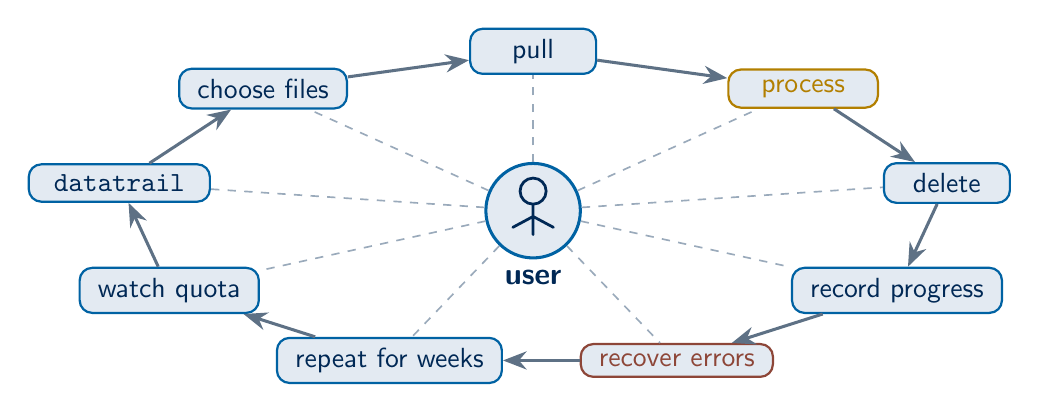
\begin{tikzpicture}[x=.92cm,y=.92cm]
    % Nine chips on a regular ellipse (40-degree pitch) around the user.
    \node[chip,minimum width=1.6cm]  (pull)    at ({7.8+5.8*cos(90)},{2.55+2.2*sin(90)})   {pull};
    \node[chipamber,minimum width=1.9cm] (process) at ({7.8+5.8*cos(50)},{2.55+2.2*sin(50)})   {process};
    \node[chip,minimum width=1.6cm]  (delete)  at ({7.8+5.8*cos(10)},{2.55+2.2*sin(10)})   {delete};
    \node[chip,minimum width=2.2cm]  (record)  at ({7.8+5.8*cos(-30)},{2.55+2.2*sin(-30)}) {record progress};
    \node[chipred,minimum width=2.0cm] (recover) at ({7.8+5.8*cos(-70)},{2.55+2.2*sin(-70)}) {recover errors};
    \node[chip,minimum width=2.2cm]  (repeat)  at ({7.8+5.8*cos(-110)},{2.55+2.2*sin(-110)}) {repeat for weeks};
    \node[chip,minimum width=2.1cm]  (quota)   at ({7.8+5.8*cos(-150)},{2.55+2.2*sin(-150)}) {watch quota};
    \node[chip,minimum width=2.3cm]  (ls)      at ({7.8+5.8*cos(170)},{2.55+2.2*sin(170)}) {\texttt{datatrail}};
    \node[chip,minimum width=2.0cm]  (choose)  at ({7.8+5.8*cos(130)},{2.55+2.2*sin(130)}) {choose files};

    \node[draw=DTCyan,line width=1.1pt,circle,minimum size=1.2cm,fill=DTPanelUp] (person) at (7.8,2.55) {};
    \draw[DTInk,line width=1pt] (7.8,2.82) circle (.18);
    \draw[DTInk,line width=1pt,line cap=round]
      (7.8,2.63)--(7.8,2.22) (7.8,2.47)--(7.52,2.32) (7.8,2.47)--(8.08,2.32);
    \node[text=DTInk,font=\fontsize{11}{13}\selectfont\bfseries] at (7.8,1.62) {user};

    \foreach \a/\b in {ls/choose,choose/pull,pull/process,process/delete,delete/record,
                       record/recover,recover/repeat,repeat/quota,quota/ls}{
      \draw[flowmuted] (\a)--(\b);
    }
    \foreach \n in {ls,choose,pull,process,delete,record,recover,repeat,quota}{
      \draw[link] (person)--(\n);
    }
  \end{tikzpicture}
  \takeaway{The per-file science is manageable; the manual loop around it hides archive navigation, storage control, and recovery in fragile ad hoc state.}
  \source{Motivating example: README ``Extending datatrawl'' --- an F-statistic detector over 23 nominal DTV pilot positions.}
  \note{
    The motivating workload was PilotProxy: apply the same F-statistic detector
    to CHIME baseband at the 23 nominal ATSC pilot positions. For any one file
    the scientific operation is well defined; the campaign is that operation
    repeated across thousands of event--channel units for weeks. This is the
    loop that surrounds it before Datatrawl. The researcher repeatedly lists
    scopes and datasets, decides which files match the science criteria, pulls
    a file, runs the calculation, deletes the local copy, records progress, and
    handles every failure. None of these steps is individually difficult. The
    problem is that the human sits at every transition, and every analysis
    reimplements the same loop slightly differently. If the session ends between
    ``process'' and ``record progress,'' the true state is ambiguous. If a file
    is unreadable, an ad hoc script may retry it forever or silently skip it.
    Datatrawl exists to make this loop explicit and testable.
  }
\end{frame}

% 4
\begin{frame}{A 200 GB allocation cannot hold an archive campaign}
  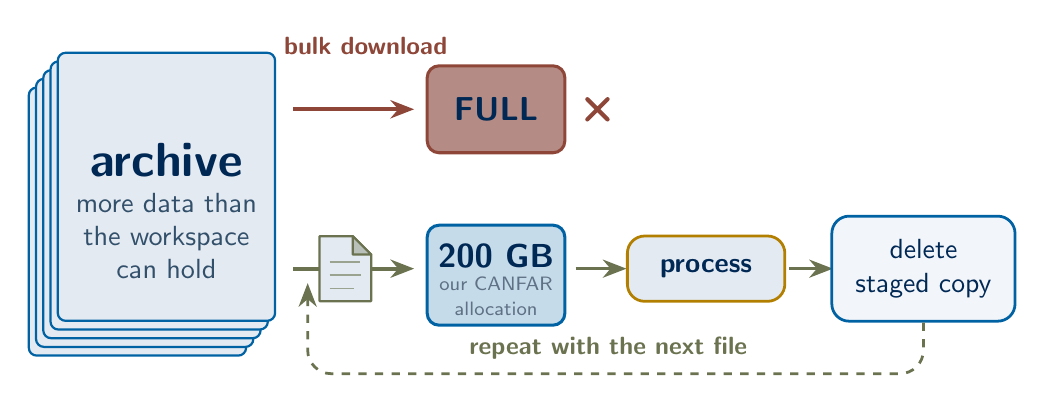
\begin{tikzpicture}[x=.92cm,y=.92cm]
    % archive stack
    \foreach \i in {0,...,4}{
      \draw[fill=DTPanelUp,draw=DTCyan,line width=.8pt,rounded corners=1mm]
        (.5+0.1*\i,0.7+0.12*\i) rectangle (3.5+0.1*\i,4.4+0.12*\i);
    }
    \node[text=DTInk,font=\fontsize{16}{19}\selectfont\bfseries] at (2.4,3.4) {archive};
    \node[smallcopy,text width=2.7cm] at (2.4,2.35)
      {more data than the workspace can hold};

    % bulk-download path (does not fit)
    \draw[flowred,strong] (4.15,4.1)--(5.82,4.1);
    \node[text=DTRed,font=\fontsize{9}{11}\selectfont\bfseries] at (5.15,4.98) {bulk download};
    \path[fill=DTRed!60!DTPanel,draw=DTRed,line width=1.1pt,rounded corners=1.5mm]
      (6.0,3.5) rectangle (7.9,4.7);
    \node[text=DTInk,font=\fontsize{12}{14}\selectfont\bfseries] at (6.95,4.1) {FULL};
    \crossicon{8.35,4.1}{DTRed}

    % streaming path (one file at a time)
    \draw[flowgreen,strong] (4.15,1.9)--(5.82,1.9);
    \fileicon[1.15]{4.87}{1.9}{DTGreen}
    \path[fill=DTCyan!18!DTPanel,draw=DTCyan,line width=1.1pt,rounded corners=1.5mm]
      (6.0,1.12) rectangle (7.9,2.5);
    \node[text=DTInk,font=\fontsize{12}{14}\selectfont\bfseries] at (6.95,2.08) {200 GB};
    \node[text=DTMuted,font=\fontsize{7.5}{9}\selectfont,align=center] at (6.95,1.52)
      {our CANFAR\\allocation};

    \draw[flowgreen] (8.05,1.9)--(8.75,1.9);
    \node[cardamber,minimum width=2.0cm] (proc) at (9.85,1.9) {\bfseries process};
    \draw[flowgreen] (11.0,1.9)--(11.6,1.9);
    \node[card,minimum width=2.2cm] (del) at (12.85,1.9) {delete\\staged copy};
    \draw[return,rounded corners=3mm] (del.south) -- (12.85,0.45) -- (4.35,0.45) -- (4.35,1.7);
    \node[text=DTGreen,font=\fontsize{9}{11}\selectfont\bfseries] at (8.5,0.8)
      {repeat with the next file};
  \end{tikzpicture}
  \takeaway{The viable model is file-granularity streaming: stage one complete file, process it, delete the staged copy, repeat.}
  \source{Project allocation: 200 GB (campaign constraint). \href{https://www.opencadc.org/canfar/latest/platform/storage/}{CANFAR Storage Systems} documents \texttt{/scratch} as temporary session storage.}
  \note{
    The second motivation is storage. Our CANFAR allocation is 200 gigabytes,
    while the selected archive campaign can be much larger. Bulk download is not
    an option. Also, for this access path we cannot consume an archive object as a
    live byte stream directly into the detector. A complete primary file must be
    staged locally first. Therefore the useful abstraction is file-granularity
    streaming: pull one file, process it, delete only the staged copy, and move to
    the next file. The bound is expressed as a number of staged files, so the
    largest selected file plus the result and checkpoint overhead still has to
    fit. The archive object is never deleted.
  }
\end{frame}

% 5
\begin{frame}{Weeks-long jobs will be interrupted}
  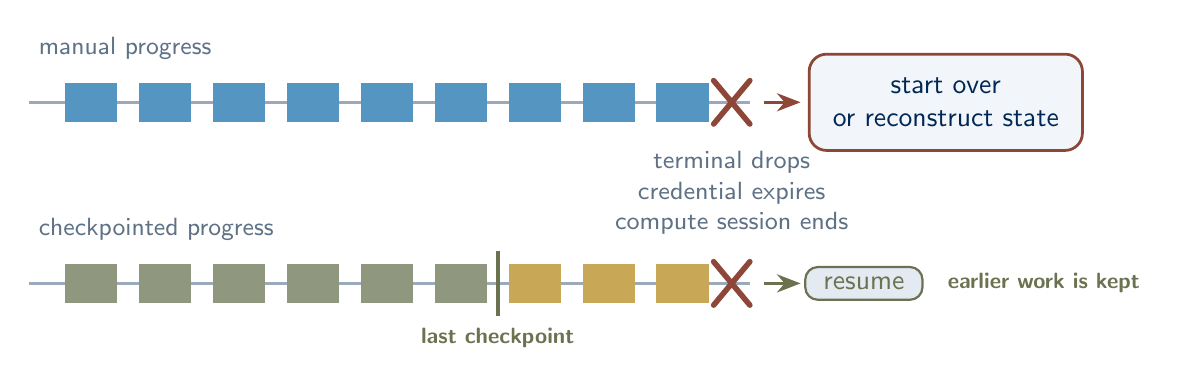
\begin{tikzpicture}[x=.92cm,y=.92cm]
    % Two timelines with identical geometry; the same interruption hits both.
    % --- manual progress ---
    \node[label,anchor=west] at (.4,5.15) {manual progress};
    \draw[DTGray,line width=1.0pt] (.4,4.4)--(10.35,4.4);
    \foreach \x in {0,...,8}{
      \fill[DTCyan!65!DTPanel] (.9+1.02*\x,4.13) rectangle ++(.72,.54);
    }
    \draw[DTRed,line width=2pt,line cap=round] (9.85,4.1)--(10.35,4.7) (10.35,4.1)--(9.85,4.7);
    \draw[flowred] (10.55,4.4)--(11.05,4.4);
    \node[cardred,anchor=west] at (11.15,4.4) {start over\\or reconstruct state};

    % --- the same interruption ---
    \node[label,text width=3.1cm] at (10.1,3.15)
      {terminal drops\\credential expires\\compute session ends};

    % --- checkpointed progress ---
    \node[label,anchor=west] at (.4,2.65) {checkpointed progress};
    \draw[DTGray,line width=1.0pt] (.4,1.9)--(10.35,1.9);
    \foreach \x in {0,...,5}{
      \fill[DTGreen!72!DTPanel] (.9+1.02*\x,1.63) rectangle ++(.72,.54);
    }
    \foreach \x in {6,...,8}{
      \fill[DTAmber!65!DTPanel] (.9+1.02*\x,1.63) rectangle ++(.72,.54);
    }
    \draw[DTGreen,line width=1.6pt] (6.87,1.45)--(6.87,2.35);
    \node[text=DTGreen,font=\fontsize{8.5}{10}\selectfont\bfseries] at (6.87,1.15) {last checkpoint};
    \draw[DTRed,line width=2pt,line cap=round] (9.85,1.6)--(10.35,2.2) (10.35,1.6)--(9.85,2.2);
    \draw[flowgreen] (10.55,1.9)--(11.05,1.9);
    \node[chipgreen,anchor=west] at (11.1,1.9) {resume};
    \node[text=DTGreen,font=\fontsize{8.5}{10}\selectfont\bfseries,anchor=west] at (12.95,1.9)
      {earlier work is kept};
  \end{tikzpicture}
  \takeaway{Progress that exists only in a running process is not durable progress.}
  \source{\href{https://github.com/WVURAIL/datatrawl/blob/6d7a239/docs/TROUBLESHOOTING.md}{docs/TROUBLESHOOTING.md}: long runs can outlive a terminal, certificate, or compute session.}
  \note{
    The third motivation is failure. A weeks-long campaign will eventually
    outlive a terminal, a credential, or a CANFAR compute session. Tmux protects
    against losing a terminal connection, but it cannot preserve a process after
    the compute session itself ends. In the upper timeline, everything that
    happened exists only in memory or in an informal log, so recovery requires
    reconstructing state and often repeating the entire job. In the lower
    timeline, completed unit keys are part of a durable scientific checkpoint.
    On restart, the engine skips those committed units. Work after the last
    checkpoint may repeat, but weeks of earlier work do not.
  }
\end{frame}

\section{Design}

% 6
\begin{frame}{Those constraints dictate the design}
  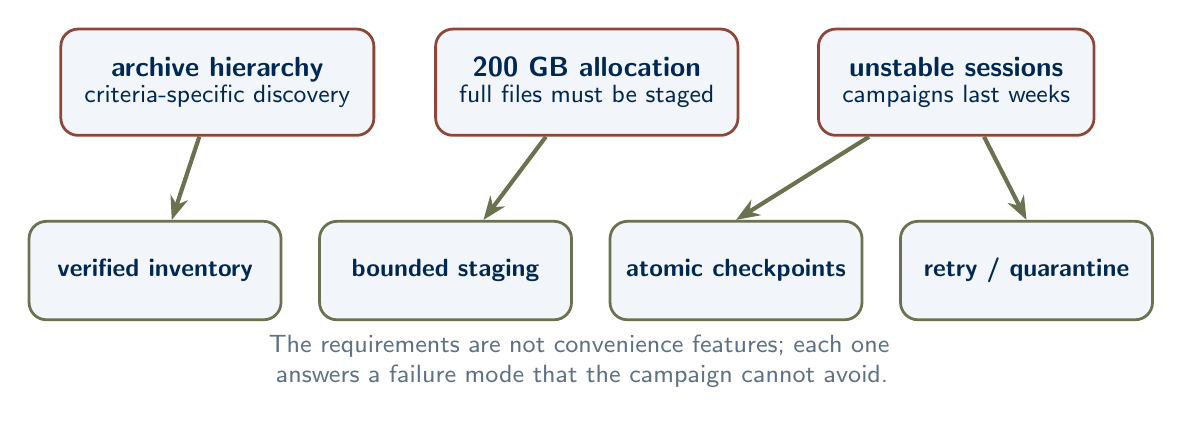
\begin{tikzpicture}[x=.92cm,y=.92cm]
    \node[cardred,minimum width=3.5cm,minimum height=1.35cm] (maze) at (2.7,4.15)
      {\bfseries archive hierarchy\\[-1mm]\fontsize{9}{11}\selectfont criteria-specific discovery};
    \node[cardred,minimum width=3.5cm,minimum height=1.35cm] (bucket) at (7.8,4.15)
      {\bfseries 200 GB allocation\\[-1mm]\fontsize{9}{11}\selectfont full files must be staged};
    \node[cardred,minimum width=3.5cm,minimum height=1.35cm] (crash) at (12.9,4.15)
      {\bfseries unstable sessions\\[-1mm]\fontsize{9}{11}\selectfont campaigns last weeks};

    \node[cardgreen,minimum width=3.2cm,minimum height=1.25cm,inner xsep=2mm,
          font=\fontsize{9.5}{11.5}\selectfont] (inv) at (1.84,1.55)
      {\bfseries verified inventory};
    \node[cardgreen,minimum width=3.2cm,minimum height=1.25cm,inner xsep=2mm,
          font=\fontsize{9.5}{11.5}\selectfont] (bound) at (5.85,1.55)
      {\bfseries bounded staging};
    \node[cardgreen,minimum width=3.2cm,minimum height=1.25cm,inner xsep=2mm,
          font=\fontsize{9.5}{11.5}\selectfont] (cp) at (9.86,1.55)
      {\bfseries atomic checkpoints};
    \node[cardgreen,minimum width=3.2cm,minimum height=1.25cm,inner xsep=2mm,
          font=\fontsize{9.5}{11.5}\selectfont] (fail) at (13.87,1.55)
      {\bfseries retry / quarantine};

    \draw[flowgreen,strong] (maze)--(inv);
    \draw[flowgreen,strong] (bucket)--(bound);
    \draw[flowgreen,strong] (crash)--(cp.north);
    \draw[flowgreen,strong] (crash)--(fail.north);

    \node[label,text width=12.6cm]
      at (7.7,.3) {The requirements are not convenience features; each one answers a failure mode that the campaign cannot avoid.};
  \end{tikzpicture}
  \takeaway{Datatrawl turns operational constraints into explicit, testable invariants.}
  \note{
    These three constraints lead directly to four requirements. Archive
    complexity requires a verified inventory. Limited disk requires an explicit
    staging bound. Interruptions require checkpoints whose replacement is atomic
    for ordinary process failure. And different kinds of failure require explicit
    retry or quarantine behavior. This is the design logic for Datatrawl. The
    tool is not a general scheduler and it is not a replacement for Datatrail.
    It is a small execution layer that enforces these invariants around a
    project-defined analyzer.
  }
\end{frame}

% 7
\begin{frame}{Datatrail maps the archive; Datatrawl runs the analysis}
  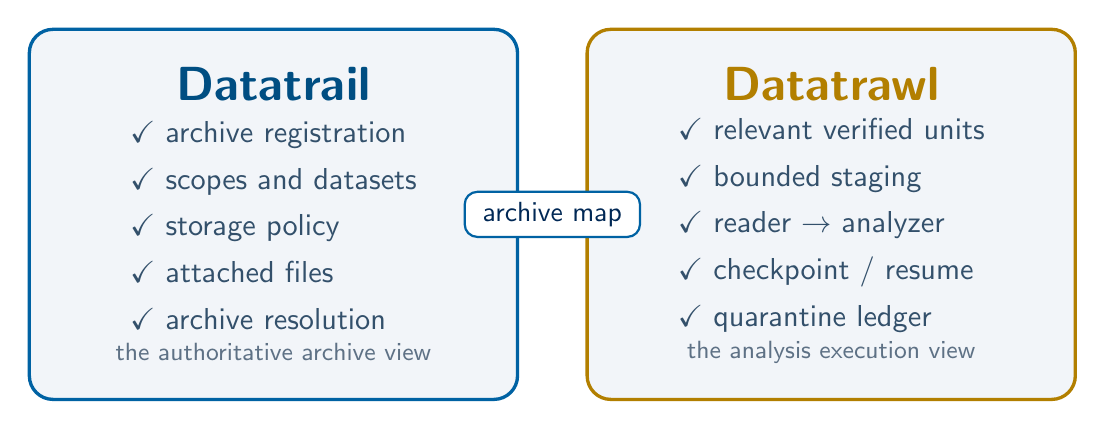
\begin{tikzpicture}[x=.92cm,y=.92cm]
    \node[panel,minimum width=6.2cm,minimum height=4.7cm] (trail) at (4.0,2.65) {};
    \node[text=DTCyanText,font=\fontsize{18}{22}\selectfont\bfseries] at (4.0,4.45) {Datatrail};
    \node[text=DTSoft,font=\fontsize{11}{14}\selectfont,align=left] at (4.0,2.5)
      {\checkmark\ archive registration\\[1mm]
       \checkmark\ scopes and datasets\\[1mm]
       \checkmark\ storage policy\\[1mm]
       \checkmark\ attached files\\[1mm]
       \checkmark\ archive resolution};
    \node[text=DTMuted,font=\fontsize{9}{11}\selectfont] at (4.0,.75) {the authoritative archive view};

    \node[panelamber,minimum width=6.2cm,minimum height=4.7cm] (trawl) at (11.7,2.65) {};
    \node[text=DTAmber,font=\fontsize{18}{22}\selectfont\bfseries] at (11.7,4.45) {Datatrawl};
    \node[text=DTSoft,font=\fontsize{11}{14}\selectfont,align=left] at (11.7,2.5)
      {\checkmark\ relevant verified units\\[1mm]
       \checkmark\ bounded staging\\[1mm]
       \checkmark\ reader $\rightarrow$ analyzer\\[1mm]
       \checkmark\ checkpoint / resume\\[1mm]
       \checkmark\ quarantine ledger};
    \node[text=DTMuted,font=\fontsize{9}{11}\selectfont] at (11.7,.75) {the analysis execution view};

    \draw[flowamber,strong] (trail.east)--(trawl.west);
    \node[chip,fill=DTCanvas] at (7.85,2.65) {archive map};
  \end{tikzpicture}
  \takeaway{Datatrail tells us what the archive contains; Datatrawl turns that view into a reliable analysis run.}
  \source{Repository boundary statement: ``datatrawl should not try to become Datatrail'' --- \href{https://github.com/WVURAIL/datatrawl/blob/6d7a239/docs/DATATRAIL_BOUNDARY.md}{DATATRAIL\_BOUNDARY.md}.}
  \note{
    The names are similar, so this boundary is worth making explicit. Datatrail
    owns the archive: registration, scopes, datasets, storage policy, and the
    files attached to a file-bearing dataset. Datatrawl consumes that view. It
    selects and verifies the units relevant to one analysis, stages them within
    a bound, passes each file through a reader and analyzer, and records durable
    progress. Datatrawl must not become another archive registry. The two tools
    are complementary: Datatrail answers ``what exists?'' and Datatrawl answers
    ``how do I finish this particular analysis safely?''
  }
\end{frame}

% 8
\begin{frame}{Discovery and execution are separate phases}
  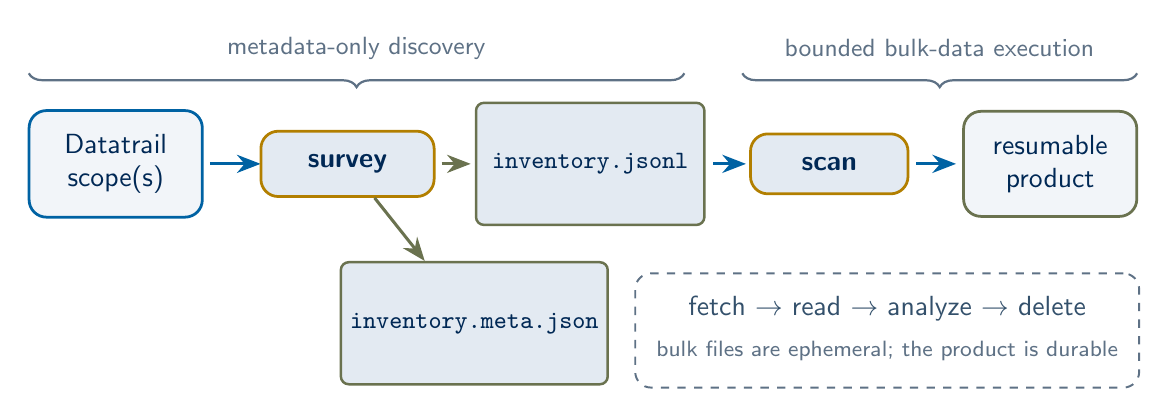
\begin{tikzpicture}[x=.92cm,y=.92cm]
    \node[card,minimum width=2.2cm] (scopes) at (1.35,3.3) {Datatrail\\scope(s)};
    \draw[flow] (2.65,3.3)--(3.35,3.3);
    \node[cardamber,minimum width=2.2cm] (survey) at (4.55,3.3) {\bfseries survey};
    \draw[flowgreen] (5.85,3.3)--(6.25,3.3);
    \node[file,draw=DTGreen,minimum width=2.9cm,minimum height=1.55cm,
          font=\fontsize{9.5}{11.5}\selectfont] (inv) at (7.9,3.3)
      {\texttt{inventory.jsonl}};
    \node[file,draw=DTGreen,minimum width=2.9cm,minimum height=1.55cm,
          font=\fontsize{9.5}{11.5}\selectfont] (meta) at (6.3,1.1)
      {\texttt{inventory.meta.json}};
    \draw[flowgreen] (survey)--(meta);

    \draw[flow] (9.6,3.3)--(10.05,3.3);
    \node[cardamber,minimum width=2.0cm] (scan) at (11.2,3.3) {\bfseries scan};
    \draw[flow] (12.4,3.3)--(12.95,3.3);
    \node[cardgreen,minimum width=2.2cm] (prod) at (14.25,3.3) {resumable\\product};

    \node[group,minimum width=6.4cm,minimum height=1.45cm] at (12.0,1.0) {};
    \node[text=DTSoft,font=\fontsize{10}{12}\selectfont] at (12.0,1.3)
      {fetch $\rightarrow$ read $\rightarrow$ analyze $\rightarrow$ delete};
    \node[sublabel] at (12.0,.72)
      {bulk files are ephemeral; the product is durable};

    \draw[decorate,decoration={brace,mirror,amplitude=5pt},DTMuted,line width=.8pt]
      (.15,4.55)--(9.2,4.55);
    \node[label] at (4.67,4.9) {metadata-only discovery};
    \draw[decorate,decoration={brace,mirror,amplitude=5pt},DTMuted,line width=.8pt]
      (10.0,4.55)--(15.45,4.55);
    \node[label] at (12.72,4.9) {bounded bulk-data execution};
  \end{tikzpicture}
  \takeaway{The exact work list is durable before the first bulk file is staged.}
  \source{Workflow and artifact names: repository README, current \texttt{master}.}
  \note{
    Datatrawl separates discovery from execution. Survey walks the selected
    Datatrail scopes and checks the expected units using archive metadata. It
    writes a JSON Lines inventory and a metadata sidecar; it does not bulk
    download the baseband collection. That inventory can be explored, reviewed,
    and reused. Scan then reads the inventory and performs the expensive phase:
    fetch, read, analyze, delete, and checkpoint. This separation is important
    for reproducibility. We know the intended work list before compute begins,
    and an archive outage during a later scan does not erase that list.
  }
\end{frame}

% 9
\begin{frame}{One fixed engine connects four interchangeable pieces}
  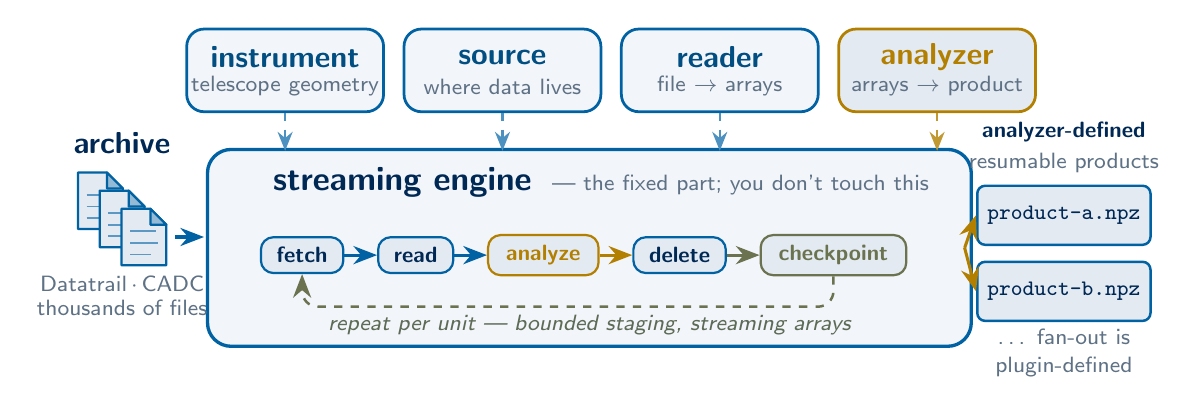
\begin{tikzpicture}[x=.92cm,y=.92cm,
      piecename/.style={text=DTCyanText,font=\fontsize{10.5}{12.5}\selectfont\bfseries},
      piecesub/.style={text=DTMuted,font=\fontsize{8}{9.5}\selectfont},
      engchip/.style={chip,inner xsep=2mm,font=\fontsize{8.5}{10}\selectfont\bfseries},
      drop/.style={-{Stealth[length=2.4mm,width=1.9mm]},DTCyan!70!DTCanvas,
                   line width=0.9pt,dashed},
      dropamber/.style={drop,DTAmber!80!DTCanvas}]

    % ------------------------------------------------ four interchangeable pieces
    \node[card,minimum width=2.5cm,minimum height=1.05cm,inner sep=2mm]      (instrument) at (3.2,4.9)  {};
    \node[card,minimum width=2.5cm,minimum height=1.05cm,inner sep=2mm]      (source)     at (6.2,4.9)  {};
    \node[card,minimum width=2.5cm,minimum height=1.05cm,inner sep=2mm]      (reader)     at (9.2,4.9)  {};
    \node[cardamber,minimum width=2.5cm,minimum height=1.05cm,inner sep=2mm] (analyzer)   at (12.2,4.9) {};
    \node[piecename] at (3.2,5.08)  {instrument};
    \node[piecesub]  at (3.2,4.68)  {telescope geometry};
    \node[piecename] at (6.2,5.08)  {source};
    \node[piecesub]  at (6.2,4.68)  {where data lives};
    \node[piecename] at (9.2,5.08)  {reader};
    \node[piecesub]  at (9.2,4.68)  {file $\rightarrow$ arrays};
    \node[piecename,text=DTAmber] at (12.2,5.08) {analyzer};
    \node[piecesub]  at (12.2,4.68) {arrays $\rightarrow$ product};

    % ------------------------------------------------------------ streaming engine
    \node[panel,minimum width=9.7cm,minimum height=2.5cm] (engine) at (7.4,2.45) {};
    \node[text=DTInk,font=\fontsize{12}{14}\selectfont\bfseries,anchor=west] at (2.9,3.35)
      {streaming engine};
    \node[sublabel,anchor=west] at (6.75,3.32)
      {--- the fixed part; you don't touch this};

    \draw[drop] (instrument.south) -- (3.2,3.79);
    \draw[drop] (source.south)     -- (6.2,3.79);
    \draw[drop] (reader.south)     -- (9.2,3.79);
    \draw[dropamber] (analyzer.south) -- (12.2,3.79);

    \node[engchip,anchor=west]                   (fetch)      at (2.85,2.35) {fetch};
    \node[engchip,right=0.45 of fetch]           (read)       {read};
    \node[engchip,chipamber,right=0.45 of read]  (analyze)    {analyze};
    \node[engchip,right=0.45 of analyze]         (delete)     {delete};
    \node[engchip,chipgreen,right=0.45 of delete] (checkpoint) {checkpoint};
    \draw[flow] (fetch)--(read);
    \draw[flow] (read)--(analyze);
    \draw[flowamber] (analyze)--(delete);
    \draw[flowgreen] (delete)--(checkpoint);
    \draw[return,line width=0.9pt,rounded corners=2mm]
      (checkpoint.south) -- ++(0,-0.42) -| (fetch.south);
    \node[text=DTGreen!75!DTSoft,font=\fontsize{8}{9.5}\selectfont\itshape] at (7.4,1.38)
      {repeat per unit --- bounded staging, streaming arrays};

    % ---------------------------------------------------------------- archive in
    \node[text=DTInk,font=\fontsize{10.5}{12.5}\selectfont\bfseries] at (0.95,3.9) {archive};
    \fileicon{0.65}{3.1}{DTCyan}
    \fileicon{0.95}{2.85}{DTCyan}
    \fileicon{1.25}{2.6}{DTCyan}
    \node[text=DTMuted,font=\fontsize{8}{9.5}\selectfont] at (0.95,1.95) {Datatrail\,$\cdot$\,CADC};
    \node[text=DTMuted,font=\fontsize{8}{9.5}\selectfont] at (0.95,1.62) {thousands of files};
    \draw[flow] (1.68,2.6)--(2.08,2.6);

    % -------------------------------------------------------------- products out
    \node[text=DTInk,font=\fontsize{8.5}{10}\selectfont\bfseries] at (13.95,4.05)
      {analyzer-defined};
    \node[sublabel] at (13.95,3.62) {resumable products};
    \node[file,minimum width=2.2cm,minimum height=0.75cm,
          font=\fontsize{8}{9.5}\selectfont] (pa) at (13.95,2.9) {\texttt{product-a.npz}};
    \node[file,minimum width=2.2cm,minimum height=0.75cm,
          font=\fontsize{8}{9.5}\selectfont] (pb) at (13.95,1.85) {\texttt{product-b.npz}};
    \node[sublabel] at (13.95,1.0) {\dots\ fan-out is\\plugin-defined};
    \draw[flowamber] (12.58,2.45)--(pa.west);
    \draw[flowamber] (12.58,2.45)--(pb.west);
  \end{tikzpicture}

  \source{This figure is the repository architecture asset (\texttt{assets/architecture.tikz}); amber denotes the analyzer supplied by the science project.}
  \note{
    This is the complete architecture. An instrument provides telescope geometry
    such as the band, channelization, feed count, Nyquist zone, and default FFT
    length. A source lists and stages data from CADC/Datatrail or from a local
    directory. A reader turns one staged file into arrays and metadata. The
    analyzer consumes those arrays and owns the scientific product. The engine
    in the middle is fixed. For each unit it fetches, reads, analyzes, deletes,
    and periodically asks the analyzer to save. Most new CHIME-compatible science
    therefore requires only a new analyzer.
  }
\end{frame}

% 10
\begin{frame}{Most pieces already exist; you write the analyzer}
  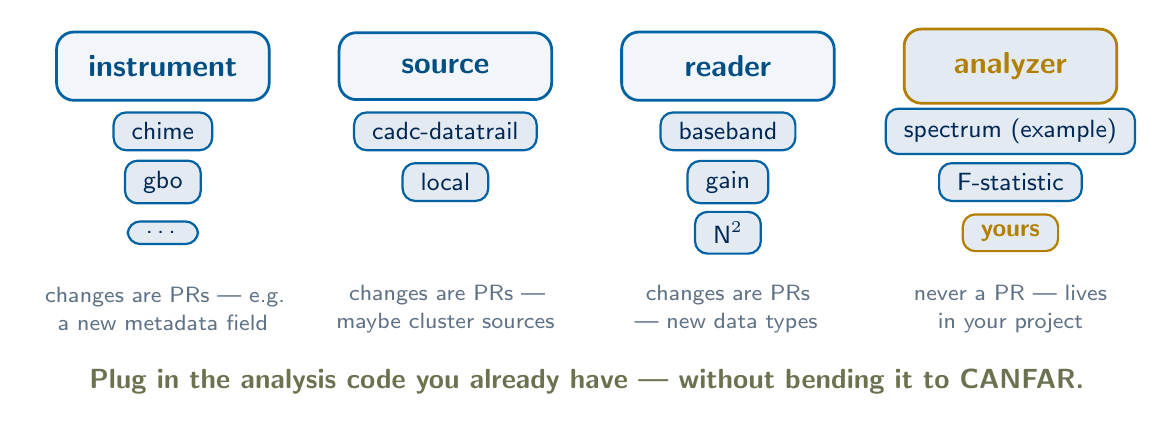
\begin{tikzpicture}[x=.92cm,y=.92cm,
      slothead/.style={card,minimum width=2.7cm,minimum height=0.85cm,
                       font=\fontsize{10.5}{12.5}\selectfont\bfseries,text=DTCyanText},
      slotchip/.style={chip,font=\fontsize{9}{11}\selectfont},
      slotnote/.style={sublabel,text width=3.2cm}]

    \node[slothead] at (2.0,4.7) {instrument};
    \node[slotchip] at (2.0,3.8) {chime};
    \node[slotchip] at (2.0,3.1) {gbo};
    \node[slotchip] at (2.0,2.4) {\dots};
    \node[slotnote] at (2.0,1.35) {changes are PRs --- e.g.\ a new metadata field};

    \node[slothead] at (5.9,4.7) {source};
    \node[slotchip] at (5.9,3.8) {cadc-datatrail};
    \node[slotchip] at (5.9,3.1) {local};
    \node[slotnote] at (5.9,1.35) {changes are PRs --- maybe cluster sources};

    \node[slothead] at (9.8,4.7) {reader};
    \node[slotchip] at (9.8,3.8) {baseband};
    \node[slotchip] at (9.8,3.1) {gain};
    \node[slotchip] at (9.8,2.4) {N$^2$};
    \node[slotnote] at (9.8,1.35) {changes are PRs --- new data types};

    \node[slothead,cardamber,text=DTAmber] at (13.7,4.7) {analyzer};
    \node[slotchip] at (13.7,3.8) {spectrum (example)};
    \node[slotchip] at (13.7,3.1) {F-statistic};
    \node[chipamber,font=\fontsize{9}{11}\selectfont\bfseries] at (13.7,2.4) {yours};
    \node[slotnote] at (13.7,1.35) {never a PR --- lives in your project};

    \node[text=DTGreen,font=\fontsize{10}{12}\selectfont\bfseries] at (7.85,0.35)
      {Plug in the analysis code you already have --- without bending it to CANFAR.};
  \end{tikzpicture}

  \takeaway{Instrument, source, and reader changes are PRs to datatrawl; the analyzer never is --- it lives in the project, by design.}
  \source{Current inventory: \texttt{datatrawl list}; plugin design: repository README.}
  \note{
    The natural worry when a tool shows four plugin slots is that a new
    project must fill all four. In practice three are already stocked, and
    changes to those three arrive as pull requests to datatrawl: instruments
    only when a new metadata field is needed, sources rarely ---
    cadc-datatrail and local today, perhaps cluster sources like fir or
    cedar someday --- and readers whenever a new data type appears;
    baseband, gain, and N-squared exist now. The analyzer is the deliberate
    exception: it lives in your project and is never a PR here. Spectrum is
    the built-in hello-world, the one analyzer that ships inside datatrawl
    so the first run works out of the box; treat it as executable
    documentation of the contract, not as an invitation to merge analyzers
    into the engine. The real starting point for a
    project is the external template repository, datatrawl-analyzer-template:
    use it as a GitHub template, rename the package, and replace the math ---
    the entry point declared in its pyproject makes your analyzer first-class
    in list, doctor, and scan. The design goal is to be unintrusive: bring the
    analysis code you have been developing, and datatrawl handles CANFAR,
    staging, and recovery without your code bending to any of it. Nobody
    swaps a working method unless trying the new one is nearly free.
  }
\end{frame}

\section{Anatomy of a run}

% 11
\begin{frame}{Survey is a filter: 23 channels across selected CHIME scopes}
  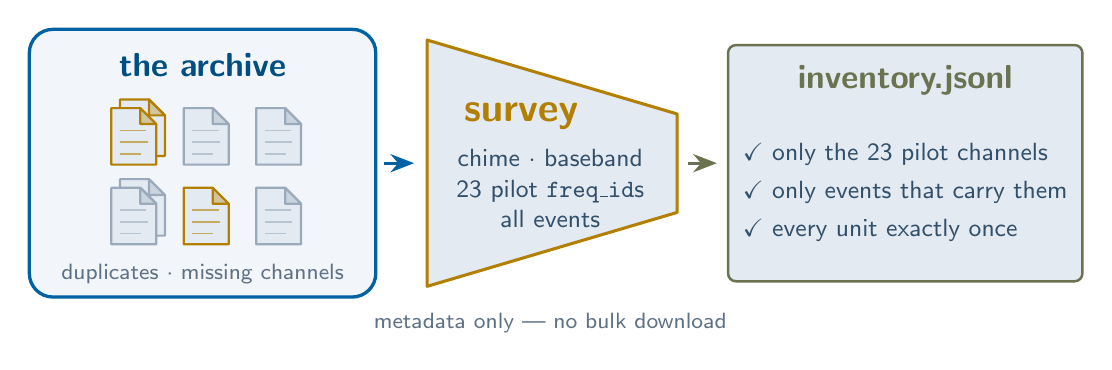
\begin{tikzpicture}[x=.92cm,y=.92cm]
    % the archive as it is: duplicates, events with partial or missing channels
    \node[panel,minimum width=4.4cm,minimum height=3.4cm] (mess) at (2.5,3.35) {};
    \node[text=DTCyanText,font=\fontsize{12}{14}\selectfont\bfseries] at (2.5,4.7) {the archive};
    \fileicon{1.67}{3.84}{DTAmber}\fileicon{1.55}{3.72}{DTAmber}% duplicate pair, wanted channel
    \fileicon{2.55}{3.72}{DTGray}
    \fileicon{3.55}{3.72}{DTGray}
    \fileicon{1.67}{2.74}{DTGray}\fileicon{1.55}{2.62}{DTGray}% duplicate pair, other channel
    \fileicon{2.55}{2.62}{DTAmber}
    \fileicon{3.55}{2.62}{DTGray}
    \node[sublabel] at (2.5,1.82) {duplicates $\cdot$ missing channels};

    \draw[flow] (5.0,3.35)--(5.42,3.35);

    % survey funnel with PilotProxy's concrete criteria
    \draw[fill=DTPanelUp,draw=DTAmber,line width=1.1pt,line join=round]
      (5.6,5.05) -- (9.05,4.03) -- (9.05,2.67) -- (5.6,1.65) -- cycle;
    \node[text=DTAmber,font=\fontsize{14}{17}\selectfont\bfseries] at (6.9,4.0) {survey};
    \node[text=DTSoft,font=\fontsize{9}{11}\selectfont,align=center] at (7.3,3.0)
      {chime $\cdot$ baseband\\23 pilot \texttt{freq\_id}s\\all events};
    \node[sublabel] at (7.3,1.15) {metadata only --- no bulk download};

    \draw[flowgreen] (9.2,3.35)--(9.6,3.35);

    % the verified work list
    \node[file,draw=DTGreen,minimum width=4.5cm,minimum height=3.0cm] (json) at (12.2,3.35) {};
    \node[text=DTGreen,font=\fontsize{12}{14}\selectfont\bfseries] at (12.2,4.5) {inventory.jsonl};
    \node[text=DTSoft,font=\fontsize{9}{11}\selectfont,align=left] at (12.2,2.95)
      {\checkmark\ only the 23 pilot channels\\[1mm]
       \checkmark\ only events that carry them\\[1mm]
       \checkmark\ every unit exactly once};
  \end{tikzpicture}

  \takeaway{Survey filters the archive down to a deduplicated, verified list of exactly the units that exist and match the criteria.}
  \source{Implementation: \texttt{src/datatrawl/plugins/sources/cadc\_datatrail.py}; inventory contract: README; pilot selection: README ``Extending datatrawl''.}
  \note{
    Survey is a filter over the archive. The PilotProxy criteria say: across
    the selected CHIME baseband scopes, keep exactly the 23 nominal DTV pilot
    channels.
    The archive does not hand over that list directly: registrations are
    duplicated, some events lack the pilot channels entirely, and others carry
    only a subset. Survey enumerates events under the selected scopes, asks
    the reader which files each event should contribute, verifies the
    candidates against archive metadata, and writes each surviving unit
    exactly once as one JSONL row: stable identity, event, file name, size,
    archive path, and shape fields such as freq-id. Duplicates collapse to a
    single unit; absent channels simply produce no row. A repeated survey tops up unfinished work;
    re-enumerate picks up newly registered events. No bulk data move in this
    phase.
  }
\end{frame}

% 12
\begin{frame}{Kevin's campaign: same survey, different criteria}
  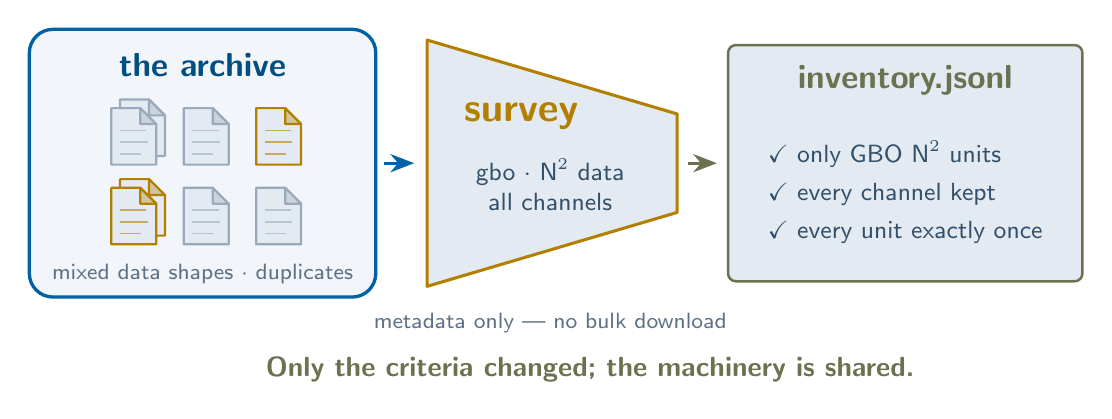
\begin{tikzpicture}[x=.92cm,y=.92cm]
    % the same archive, a different mess dimension
    \node[panel,minimum width=4.4cm,minimum height=3.4cm] (mess) at (2.5,3.35) {};
    \node[text=DTCyanText,font=\fontsize{12}{14}\selectfont\bfseries] at (2.5,4.7) {the archive};
    \fileicon{1.67}{3.84}{DTGray}\fileicon{1.55}{3.72}{DTGray}% duplicate pair, other shape
    \fileicon{2.55}{3.72}{DTGray}
    \fileicon{3.55}{3.72}{DTAmber}
    \fileicon{1.67}{2.74}{DTAmber}\fileicon{1.55}{2.62}{DTAmber}% duplicate pair, wanted shape
    \fileicon{2.55}{2.62}{DTGray}
    \fileicon{3.55}{2.62}{DTGray}
    \node[sublabel] at (2.5,1.82) {mixed data shapes $\cdot$ duplicates};

    \draw[flow] (5.0,3.35)--(5.42,3.35);

    % the same funnel, Kevin's criteria
    \draw[fill=DTPanelUp,draw=DTAmber,line width=1.1pt,line join=round]
      (5.6,5.05) -- (9.05,4.03) -- (9.05,2.67) -- (5.6,1.65) -- cycle;
    \node[text=DTAmber,font=\fontsize{14}{17}\selectfont\bfseries] at (6.9,4.0) {survey};
    \node[text=DTSoft,font=\fontsize{9}{11}\selectfont,align=center] at (7.3,3.05)
      {gbo $\cdot$ N$^2$ data\\all channels};
    \node[sublabel] at (7.3,1.15) {metadata only --- no bulk download};

    \draw[flowgreen] (9.2,3.35)--(9.6,3.35);

    % its own verified work list
    \node[file,draw=DTGreen,minimum width=4.5cm,minimum height=3.0cm] (json) at (12.2,3.35) {};
    \node[text=DTGreen,font=\fontsize{12}{14}\selectfont\bfseries] at (12.2,4.5) {inventory.jsonl};
    \node[text=DTSoft,font=\fontsize{9}{11}\selectfont,align=left] at (12.2,2.95)
      {\checkmark\ only GBO N$^2$ units\\[1mm]
       \checkmark\ every channel kept\\[1mm]
       \checkmark\ every unit exactly once};

    \node[text=DTGreen,font=\fontsize{10}{12}\selectfont\bfseries] at (7.85,0.5)
      {Only the criteria changed; the machinery is shared.};
  \end{tikzpicture}
  \takeaway{A second campaign is the same survey command with different criteria; enumeration, verification, and dedup are shared.}
  \note{
    Kevin's campaign asks the opposite question: keep every channel, but only
    GBO N-squared correlation data rather than CHIME baseband. The command is
    the same survey with different criteria: the instrument is gbo, the
    reader matches the N-squared file shape, and no channel selection is
    applied. The archive mess is the same mess --- duplicated registrations
    and mixed data shapes --- and the same machinery absorbs it: enumeration,
    verification against archive metadata, one row per surviving unit, and
    resumable survey state. Each campaign keeps its own named inventory, so
    the two work lists never interfere. With the GBO instrument and reader
    pieces registered, nothing else in the engine changes.
  }
\end{frame}

% 13
\begin{frame}{Explore estimates the campaign before data move}
  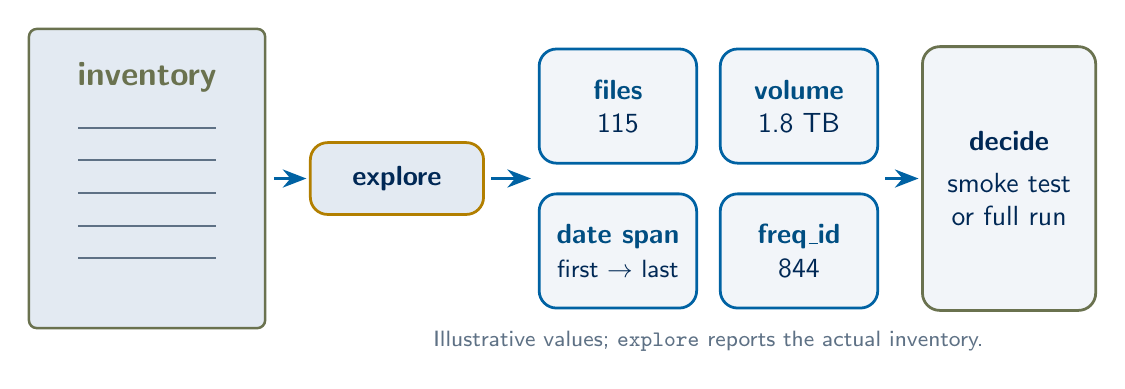
\begin{tikzpicture}[x=.92cm,y=.92cm]
    \node[file,draw=DTGreen,minimum width=3.0cm,minimum height=3.8cm] (inv) at (2.3,2.85) {};
    \node[text=DTGreen,font=\fontsize{13}{16}\selectfont\bfseries] at (2.3,4.25) {inventory};
    \foreach \y in {1.75,2.2,2.65,3.1,3.55}{
      \draw[DTMuted,line width=.7pt] (1.35,\y)--(3.25,\y);
    }
    \draw[flow] (4.05,2.85)--(4.5,2.85);
    \node[cardamber,minimum width=2.2cm] (explore) at (5.75,2.85) {\bfseries explore};
    \draw[flow] (7.05,2.85)--(7.6,2.85);

    \node[card,minimum width=2.0cm,minimum height=1.45cm,inner xsep=2mm] at (8.8,3.85)
      {\textcolor{DTCyanText}{\bfseries files}\\\fontsize{10}{12}\selectfont 115};
    \node[card,minimum width=2.0cm,minimum height=1.45cm,inner xsep=2mm] at (11.3,3.85)
      {\textcolor{DTCyanText}{\bfseries volume}\\\fontsize{10}{12}\selectfont 1.8 TB};
    \node[card,minimum width=2.0cm,minimum height=1.45cm,inner xsep=2mm] at (8.8,1.85)
      {\textcolor{DTCyanText}{\bfseries date span}\\\fontsize{9.5}{11}\selectfont first $\rightarrow$ last};
    \node[card,minimum width=2.0cm,minimum height=1.45cm,inner xsep=2mm] at (11.3,1.85)
      {\textcolor{DTCyanText}{\bfseries freq\_id}\\\fontsize{10}{12}\selectfont 844};
    \draw[flow] (12.49,2.85)--(12.95,2.85);
    \node[cardgreen,minimum width=2.2cm,minimum height=3.35cm] at (14.2,2.85)
      {\bfseries decide\\[1mm]\fontsize{10}{12}\selectfont smoke test\\or full run};
    \node[sublabel] at (10.05,0.6)
      {Illustrative values; \texttt{explore} reports the actual inventory.};
  \end{tikzpicture}
  \takeaway{A lightweight inventory reveals scope and cost before any expensive staging begins.}
  \note{
    Explore is a small but important step between survey and scan ---
    strictly optional, since only survey and scan are required, but in
    practice we inspect the inventory before spending compute. It reads the
    inventory and reports which frequency IDs are present, the number of files,
    the date span, and the total volume. The numbers on this slide are only
    illustrative; the command prints the actual values for the named inventory.
    This lets us detect a wrong selection or an unexpectedly large campaign
    before allocating a GPU or moving bulk data. It also makes a bounded smoke
    test a deliberate choice rather than an emergency response after the disk
    fills.
  }
\end{frame}

% 14
\begin{frame}{A stable unit key is the thread through the system}
  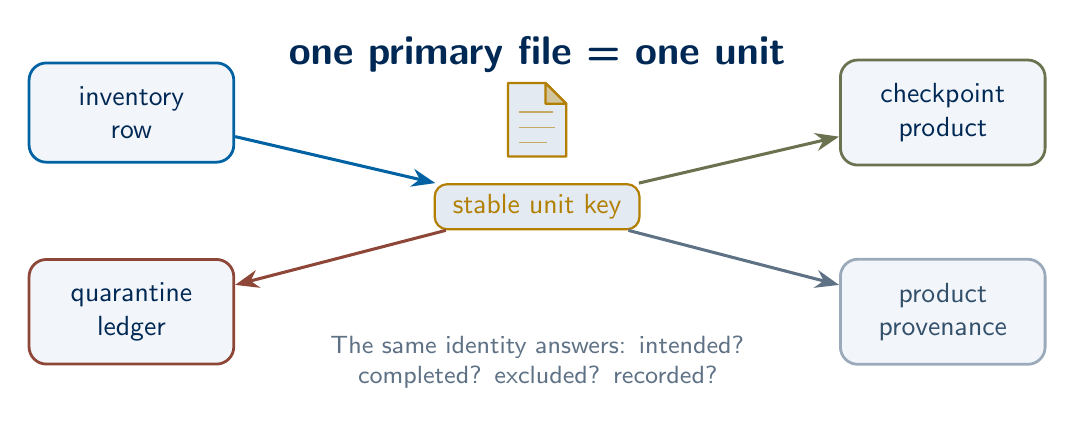
\begin{tikzpicture}[x=.92cm,y=.92cm]
    \node[biglabel] at (7.8,4.7) {one primary file = one unit};
    \fileicon[1.3]{7.8}{3.8}{DTAmber}
    \node[chipamber,minimum width=2.5cm] (key) at (7.8,2.6) {stable unit key};

    \node[card,minimum width=2.6cm] (inventory) at (2.2,3.9) {inventory\\row};
    \node[cardgreen,minimum width=2.6cm] (product) at (13.4,3.9) {checkpoint\\product};
    \node[cardred,minimum width=2.6cm] (quarantine) at (2.2,1.15) {quarantine\\ledger};
    \node[cardmuted,minimum width=2.6cm] (provenance) at (13.4,1.15) {product\\provenance};

    \draw[flow] (inventory)--(key);
    \draw[flowgreen] (key)--(product);
    \draw[flowred] (key)--(quarantine);
    \draw[flowmuted] (key)--(provenance);

    \node[label,text width=8cm] at (7.8,0.45)
      {The same identity answers: intended? completed? excluded? recorded?};
  \end{tikzpicture}
  \takeaway{The unit key connects discovery, completion, quarantine, provenance, and resume.}
  \source{Engine unit model: \texttt{src/datatrawl/interfaces.py} and \texttt{pipeline.py}.}
  \note{
    The engine needs one unambiguous identity for every unit of work. In the
    current model, a unit is one primary file. Its stable key appears in the
    inventory, in the completed-unit list stored with the product, and in the
    quarantine ledger when the source provides a stable logical quarantine key.
    This is what lets the engine ask four exact questions on restart: Was this
    unit intended? Is it already committed to the product? Was it explicitly
    excluded as unreadable? And is its identity preserved for provenance? An
    analysis that requires several bulk primary files simultaneously needs a
    different unit model; Datatrawl deliberately does not pretend otherwise.
  }
\end{frame}

% 15
\begin{frame}{Scan is a pull--process--delete conveyor}
  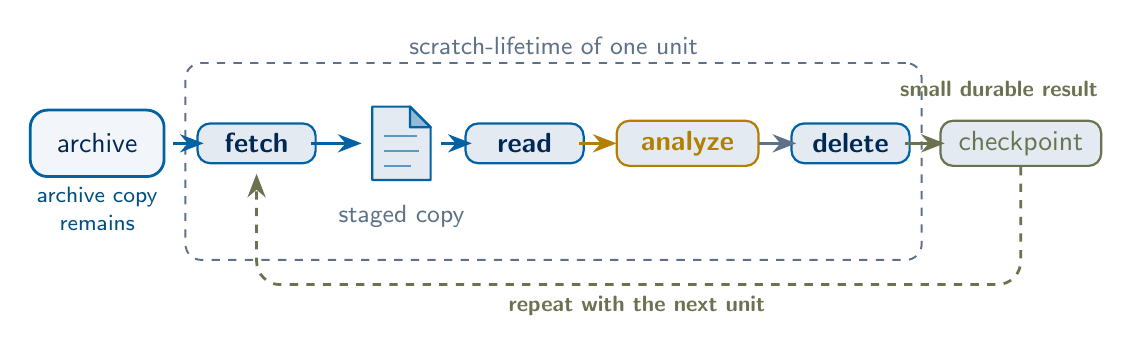
\begin{tikzpicture}[x=.92cm,y=.92cm]
    % conveyor: archive -> fetch -> staged copy -> read -> analyze -> delete -> checkpoint
    \node[group,minimum width=9.35cm,minimum height=2.5cm] (scratch) at (7.45,2.85) {};
    \node[label] at (7.45,4.45) {scratch-lifetime of one unit};

    \node[card,minimum width=1.7cm] (archive) at (1.15,3.1) {archive};
    \node[chip,minimum width=1.5cm] (fetch) at (3.35,3.1) {\bfseries fetch};
    \fileicon[1.3]{5.35}{3.1}{DTCyan}
    \node[label] at (5.35,2.1) {staged copy};
    \node[chip,minimum width=1.5cm] (read) at (7.05,3.1) {\bfseries read};
    \node[chipamber,minimum width=1.8cm] (analyze) at (9.3,3.1) {\bfseries analyze};
    \node[chip,minimum width=1.5cm] (delete) at (11.55,3.1) {\bfseries delete};
    \node[chipgreen,minimum width=1.9cm] (checkpoint) at (13.9,3.1) {checkpoint};

    \draw[flow] (2.2,3.1)--(2.62,3.1);
    \draw[flow] (4.1,3.1)--(4.8,3.1);
    \draw[flow] (5.9,3.1)--(6.32,3.1);
    \draw[flowamber] (7.8,3.1)--(8.32,3.1);
    \draw[flowmuted] (10.28,3.1)--(10.8,3.1);
    \draw[flowgreen] (12.3,3.1)--(12.85,3.1);
    \draw[return,rounded corners=3mm]
      (checkpoint.south) -- (13.9,1.15) -- (3.35,1.15) -- (3.35,2.68);
    \node[text=DTGreen,font=\fontsize{8.5}{10}\selectfont\bfseries] at (8.6,0.85)
      {repeat with the next unit};

    \node[text=DTCyanText,font=\fontsize{8.5}{10}\selectfont,align=center] at (1.15,2.2)
      {archive copy\\remains};
    \node[text=DTGreen,font=\fontsize{8.5}{10}\selectfont\bfseries] at (13.6,3.85)
      {small durable result};
  \end{tikzpicture}

  \takeaway{Bulk data are temporary; the accumulated scientific product is durable.}
  \source{Fixed loop: \texttt{src/datatrawl/pipeline.py}.}
  \note{
    Scan is the core execution loop. A downloader stages one complete primary
    file. The reader probes it and iterates arrays. The analyzer consumes those
    arrays and updates a compact scientific accumulator. In a finally block the
    engine removes the staged path, and only then releases the scratch slot for
    the next download. At the configured interval the engine asks the analyzer
    to save its product. Datatrawl deletes only the copy that it staged into its
    scratch directory. It does not delete the archive object, and the local
    source does not delete the user's original local file.
  }
\end{frame}

% 16
\begin{frame}{The scratch bound is explicit}
  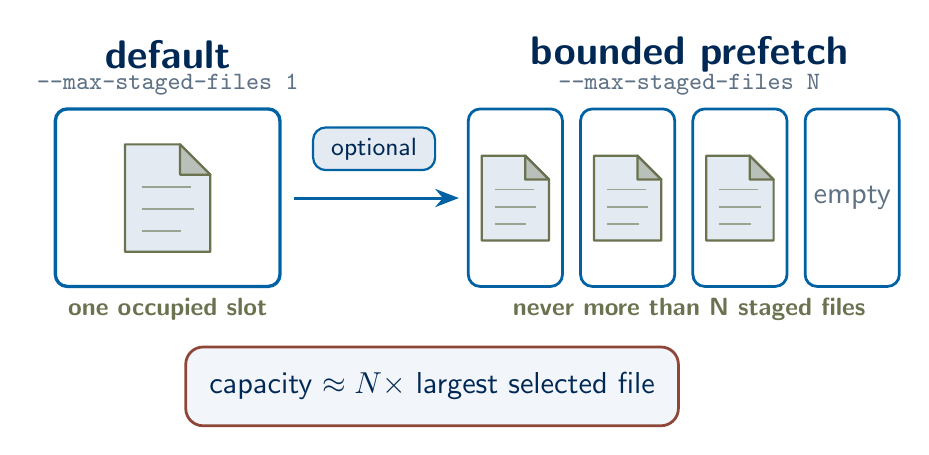
\begin{tikzpicture}[x=.92cm,y=.92cm]
    \node[text=DTInk,font=\fontsize{14}{17}\selectfont\bfseries] at (4.1,4.6) {default};
    \node[label] at (4.1,4.18) {\texttt{--max-staged-files 1}};
    \draw[slot,line width=1.2pt] (2.55,1.4) rectangle (5.65,3.85);
    \fileicon[1.9]{4.1}{2.62}{DTGreen}
    \node[text=DTGreen,font=\fontsize{9}{11}\selectfont\bfseries] at (4.1,1.08) {one occupied slot};

    \node[text=DTInk,font=\fontsize{14}{17}\selectfont\bfseries] at (11.3,4.6) {bounded prefetch};
    \node[label] at (11.3,4.18) {\texttt{--max-staged-files N}};
    \foreach \x in {0,...,3}{
      \draw[slot] (8.25+1.55*\x,1.4) rectangle (9.55+1.55*\x,3.85);
    }
    \foreach \x in {0,...,2}{
      \fileicon[1.5]{8.9+1.55*\x}{2.62}{DTGreen}
    }
    \node[text=DTMuted,font=\fontsize{11}{13}\selectfont] at (13.55,2.62) {empty};
    \node[text=DTGreen,font=\fontsize{9}{11}\selectfont\bfseries] at (11.3,1.08) {never more than N staged files};

    \draw[flow] (5.85,2.62)--(8.12,2.62);
    \node[chip,font=\fontsize{9}{11}\selectfont] at (6.95,3.3) {optional};

    \node[cardred,minimum width=4.6cm,minimum height=1.0cm] at (7.75,.02)
      {\fontsize{10.5}{13}\selectfont capacity $\approx N\times$ largest selected file};
  \end{tikzpicture}

  \takeaway{A semaphore is acquired before fetch and released only after deletion, so file count cannot exceed the configured bound.}
  \source{Defaults and semaphore behavior: \texttt{pipeline.py}; CLI help: \texttt{--download-workers 1}, \texttt{--max-staged-files 1}.}
  \note{
    The storage guarantee is enforced with a bounded semaphore. A downloader
    acquires a slot before it fetches a file. The consumer releases that slot
    only after the staged file has been deleted. With the defaults, one download
    worker and one slot, exactly one file is held at a time and source order is
    preserved. Increasing both workers and slots can overlap download and
    analysis, but the analyzer must be order-insensitive. The bound is in file
    count, not bytes. For N slots, plan space for roughly N times the largest
    selected file, plus the compact product and ordinary overhead.
  }
\end{frame}

% 17
\begin{frame}{Checkpoints turn completed units into durable progress}
  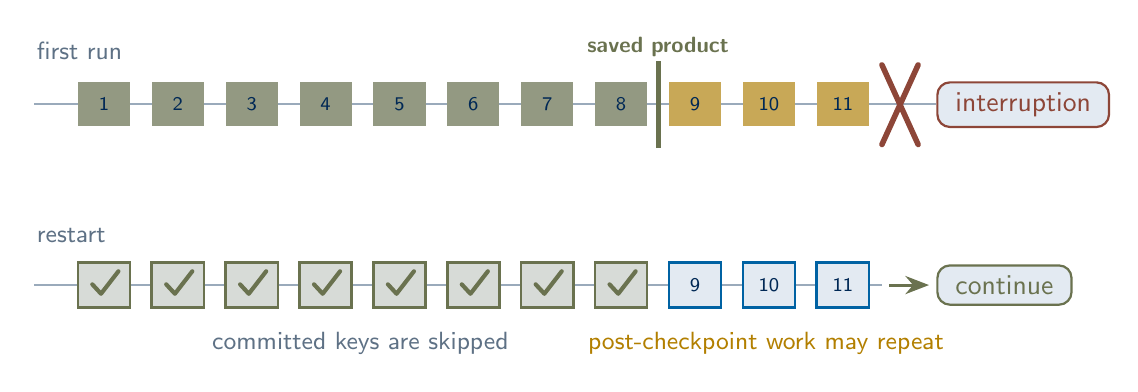
\begin{tikzpicture}[x=.92cm,y=.92cm]
    \node[label,anchor=west] at (.4,4.7) {first run};
    \draw[DTGray,line width=1.0pt] (.5,3.96)--(12.95,3.96);
    \foreach \x in {0,...,7}{
      \fill[DTGreen!70!DTPanel] (1.1+1.02*\x,3.65) rectangle ++(.72,.62);
      \node[text=DTInk,font=\fontsize{7.5}{9}\selectfont] at (1.46+1.02*\x,3.96) {\number\numexpr\x+1\relax};
    }
    \foreach \x in {8,...,10}{
      \fill[DTAmber!65!DTPanel] (1.1+1.02*\x,3.65) rectangle ++(.72,.62);
      \node[text=DTInk,font=\fontsize{7.5}{9}\selectfont] at (1.46+1.02*\x,3.96) {\number\numexpr\x+1\relax};
    }
    \draw[DTGreen,line width=1.8pt] (9.11,3.35)--(9.11,4.55);
    \node[text=DTGreen,font=\fontsize{8.5}{10}\selectfont\bfseries] at (9.11,4.75) {saved product};
    \draw[DTRed,line width=2pt,line cap=round] (12.2,3.4)--(12.7,4.5) (12.7,3.4)--(12.2,4.5);
    \node[chipred,anchor=west,font=\fontsize{10}{12}\selectfont] at (12.95,3.95) {interruption};

    \node[label,anchor=west] at (.4,2.15) {restart};
    \draw[DTGray,line width=1.0pt] (.5,1.46)--(12.2,1.46);
    \foreach \x in {0,...,7}{
      \draw[draw=DTGreen,line width=.9pt,fill=DTGreen!20!DTPanel]
        (1.1+1.02*\x,1.15) rectangle ++(.72,.62);
      \checkmarkicon{1.46+1.02*\x,1.45}{DTGreen}
    }
    \foreach \x in {8,...,10}{
      \draw[draw=DTCyan,line width=.9pt,fill=DTPanelUp]
        (1.1+1.02*\x,1.15) rectangle ++(.72,.62);
      \node[text=DTInk,font=\fontsize{7.5}{9}\selectfont] at (1.46+1.02*\x,1.46) {\number\numexpr\x+1\relax};
    }
    \draw[flowgreen] (12.3,1.46)--(12.85,1.46);
    \node[chipgreen,anchor=west,font=\fontsize{10}{12}\selectfont] at (12.95,1.46) {continue};
    \node[text=DTMuted,font=\fontsize{9}{11}\selectfont] at (5.0,.65) {committed keys are skipped};
    \node[text=DTAmber,font=\fontsize{9}{11}\selectfont] at (10.6,.65) {post-checkpoint work may repeat};
  \end{tikzpicture}

  \takeaway{Resume starts from the last safely saved product, not the last CPU instruction.}
  \source{Default request: checkpoint every 50 successfully consumed files and at normal completion; atomic NPZ replacement: \texttt{analyzer\_base.py}.}
  \note{
    A checkpoint contains both the scientific accumulators and the unit keys
    already committed to that product. The engine asks the analyzer to save every
    fifty successfully consumed files by default, and again at normal completion
    when new work was consumed. The supplied accumulating base class writes a
    temporary NPZ and replaces the prior checkpoint atomically for ordinary
    process interruption. On restart, the analyzer loads the product and reports
    the committed keys. Those units are skipped. Work performed after the last
    checkpoint can repeat, which is why the checkpoint interval trades less redo
    against more output I/O. External analyzers must honor the same save and
    resume contract.
  }
\end{frame}

% 18
\begin{frame}{Failures remain honest about what was completed}
  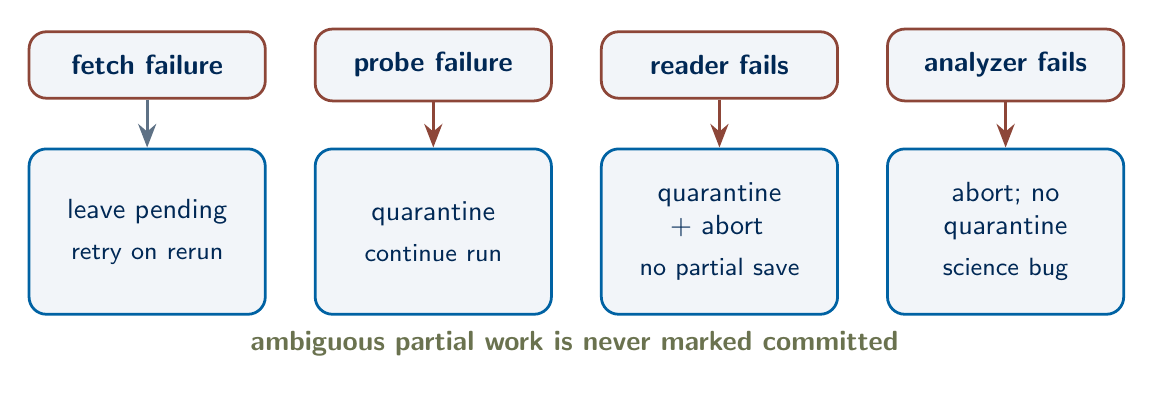
\begin{tikzpicture}[x=.92cm,y=.92cm]
    \node[cardred,minimum width=3.0cm] (fetch) at (2.0,4.1) {\bfseries fetch failure};
    \node[cardred,minimum width=3.0cm] (probe) at (5.95,4.1) {\bfseries probe failure};
    \node[cardred,minimum width=3.0cm] (reader) at (9.9,4.1) {\bfseries reader fails};
    \node[cardred,minimum width=3.0cm] (analyzer) at (13.85,4.1) {\bfseries analyzer fails};

    \node[card,minimum width=3.0cm,minimum height=2.1cm,text width=2.35cm] (fout) at (2.0,1.8)
      {leave pending\\[1mm]\fontsize{9}{11}\selectfont retry on rerun};
    \node[card,minimum width=3.0cm,minimum height=2.1cm,text width=2.35cm] (pout) at (5.95,1.8)
      {quarantine\\[1mm]\fontsize{9}{11}\selectfont continue run};
    \node[card,minimum width=3.0cm,minimum height=2.1cm,text width=2.35cm] (rout) at (9.9,1.8)
      {quarantine + abort\\[1mm]\fontsize{9}{11}\selectfont no partial save};
    \node[card,minimum width=3.0cm,minimum height=2.1cm,text width=2.35cm] (aout) at (13.85,1.8)
      {abort; no quarantine\\[1mm]\fontsize{9}{11}\selectfont science bug};

    \draw[flowmuted] (fetch)--(fout);
    \draw[flowred] (probe)--(pout);
    \draw[flowred] (reader)--(rout);
    \draw[flowred] (analyzer)--(aout);

    \node[text=DTGreen,font=\fontsize{10}{12}\selectfont\bfseries] at (7.9,.25)
      {ambiguous partial work is never marked committed};
  \end{tikzpicture}
  \takeaway{Recovery behavior depends on what failed; Datatrawl does not turn uncertainty into false completion.}
  \source{Failure semantics: \texttt{src/datatrawl/pipeline.py}. Quarantine means ``excluded from automatic reruns,'' not proof of permanent corruption.}
  \note{
    Not every failure means the same thing. A fetch failure can be transient, so
    the unit remains pending and will be retried on the next identical command.
    If the bytes arrive but the initial probe cannot read the file, the file is
    recorded in the quarantine ledger and the run continues. If the reader fails
    while yielding arrays, the file is quarantined and the run aborts without
    saving the current in-memory analyzer state. An analyzer exception is treated
    as a science or implementation error: the run aborts, the file is not
    quarantined, and unsaved in-memory state is discarded. In every case, a unit
    is committed only through a valid checkpoint.
  }
\end{frame}

% 19
\begin{frame}{The analyzer contains the science --- and the resume contract}
  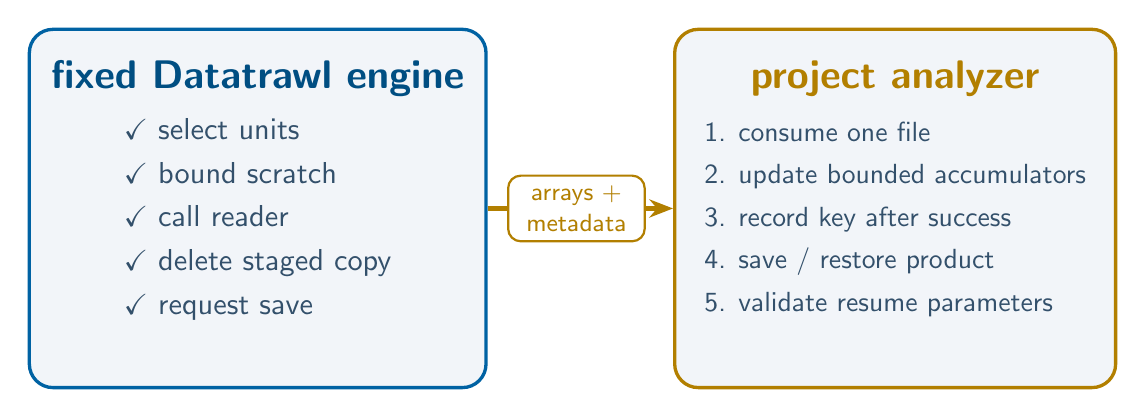
\begin{tikzpicture}[x=.92cm,y=.92cm]
    \node[panel,minimum width=5.8cm,minimum height=4.55cm] (engine) at (3.55,2.7) {};
    \node[panelhead] at (3.55,4.5) {fixed Datatrawl engine};
    \node[text=DTSoft,font=\fontsize{10.5}{13}\selectfont,align=left] at (3.55,2.55)
      {\checkmark\ select units\\[1mm]
       \checkmark\ bound scratch\\[1mm]
       \checkmark\ call reader\\[1mm]
       \checkmark\ delete staged copy\\[1mm]
       \checkmark\ request save};

    \node[panelamber,minimum width=5.6cm,minimum height=4.55cm] (analyzer) at (12.35,2.7) {};
    \node[panelhead,text=DTAmber] at (12.35,4.5) {project analyzer};
    \node[text=DTSoft,font=\fontsize{10.2}{12.5}\selectfont,align=left] at (12.35,2.55)
      {1. consume one file\\[1mm]
       2. update bounded accumulators\\[1mm]
       3. record key after success\\[1mm]
       4. save / restore product\\[1mm]
       5. validate resume parameters};

    \draw[flowamber,strong] (engine.east)--(analyzer.west);
    \node[chipamber,fill=DTCanvas,font=\fontsize{9}{11}\selectfont] at (7.95,2.7)
      {arrays +\\metadata};
  \end{tikzpicture}
  \takeaway{The scientist supplies the calculation while honoring a small, explicit resumability contract.}
  \source{Analyzer guide: \href{https://github.com/WVURAIL/datatrawl/blob/6d7a239/docs/ADDING_AN_ANALYZER.md}{docs/ADDING\_AN\_ANALYZER.md}; base class: \texttt{analyzer\_base.py}.}
  \note{
    The analyzer is the seam between shared operations and project science. It
    receives arrays and file metadata, updates bounded accumulators, and records
    the unit key only after that file has been consumed successfully. It must be
    able to save and restore its product. It should also stamp and validate every
    parameter that changes the meaning of the result. The built-in spectrum
    analyzer, for example, refuses to resume across a different frequency ID,
    sample rate, FFT length, Nyquist zone, or per-file frame cap. A thresholded
    detector should do the same for its threshold and other scientific knobs.
    The base class supplies atomic replacement and processed-key tracking,
    and the external analyzer template packages all of this as a
    ready-to-clone project with the entry point declared and tests included.
  }
\end{frame}

% 20
\begin{frame}{Your analyzer starts from working code}
  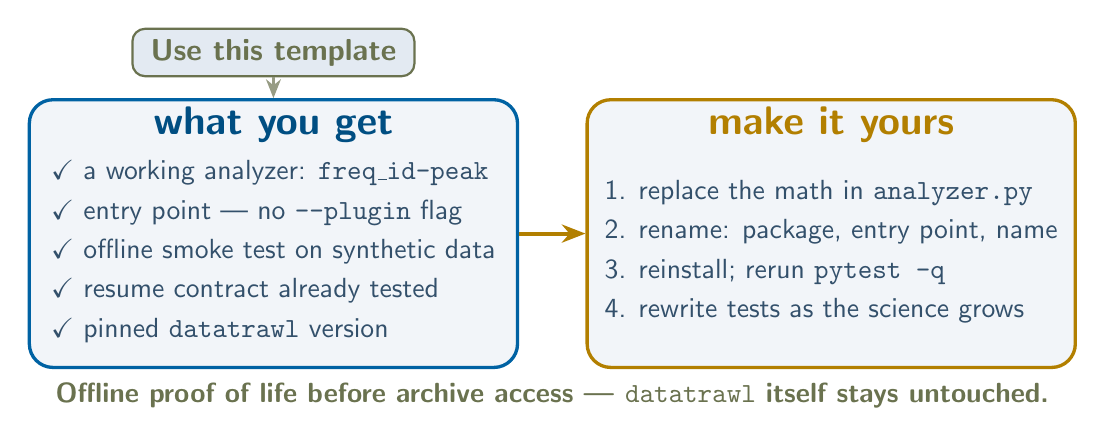
\begin{tikzpicture}[x=.92cm,y=.92cm]
    \node[chipgreen,font=\fontsize{10.5}{12.5}\selectfont\bfseries] (btn) at (4.0,4.95)
      {Use this template};
    \draw[-{Stealth[length=2.4mm,width=1.9mm]},DTGreen!70!DTCanvas,line width=0.9pt,dashed]
      (btn.south) -- (4.0,4.32);

    \node[panel,minimum width=6.2cm,minimum height=3.4cm] (get) at (4.0,2.45) {};
    \node[panelhead] at (4.0,3.95) {what you get};
    \node[text=DTSoft,font=\fontsize{10}{12.5}\selectfont,align=left] at (4.0,2.2)
      {\checkmark\ a working analyzer: \texttt{freq\_id-peak}\\[0.6mm]
       \checkmark\ entry point --- no \texttt{--plugin} flag\\[0.6mm]
       \checkmark\ offline smoke test on synthetic data\\[0.6mm]
       \checkmark\ resume contract already tested\\[0.6mm]
       \checkmark\ pinned \texttt{datatrawl} version};

    \node[panelamber,minimum width=6.2cm,minimum height=3.4cm] (yours) at (11.7,2.45) {};
    \node[panelhead,text=DTAmber] at (11.7,3.95) {make it yours};
    \node[text=DTSoft,font=\fontsize{10}{12.5}\selectfont,align=left] at (11.7,2.2)
      {1. replace the math in \texttt{analyzer.py}\\[0.6mm]
       2. rename: package, entry point, name\\[0.6mm]
       3. reinstall; rerun \texttt{pytest -q}\\[0.6mm]
       4. rewrite tests as the science grows};

    \draw[flowamber,strong] (get.east)--(yours.west);

    \node[text=DTGreen,font=\fontsize{10}{12}\selectfont\bfseries] at (7.85,0.22)
      {Offline proof of life before archive access --- \texttt{datatrawl} itself stays untouched.};
  \end{tikzpicture}
  \takeaway{Use the template, prove it offline, replace the math; the test harness --- synthesize, scan, rerun, refuse --- is the part worth keeping.}
  \source{\href{https://github.com/WVURAIL/datatrawl-analyzer-template}{WVURAIL/datatrawl-analyzer-template}: \texttt{freq\_id-peak} example, entry-point registration, engine smoke tests, pinned \texttt{datatrawl}.}
  \note{
    The template inverts the usual plugin experience: instead of an empty
    scaffold, it is a complete working analyzer that you gradually turn into
    yours. One click on Use this template copies it into your own repository.
    What you get already passes its tests: freq-id-peak computes an averaged
    power spectrum and its peak bin per freq-id, reads a parameter from
    \texttt{--set}, and stamps every meaning-changing parameter into the
    product so an incompatible rerun is refused. pip install -e is the whole
    integration --- the entry point in pyproject makes the analyzer
    first-class in list, doctor, and scan with no \texttt{--plugin} flag ---
    and pytest -q pushes synthetic
    CHIME baseband with a known tone through the real engine, so the proof of
    life happens offline, before any archive access. Making it yours is
    science first, rename second: replace the math in analyzer.py; rename
    the package, entry point, and plugin name; reinstall; and keep the test
    harness --- synthesize, scan, rerun, refuse --- rewriting its assertions
    as the science outgrows the tone. The pinned datatrawl version in
    pyproject is the compatibility contract: bump it deliberately and rerun
    the tests.
  }
\end{frame}

% 21
\begin{frame}{For PilotProxy, the archive machinery is already reusable}
  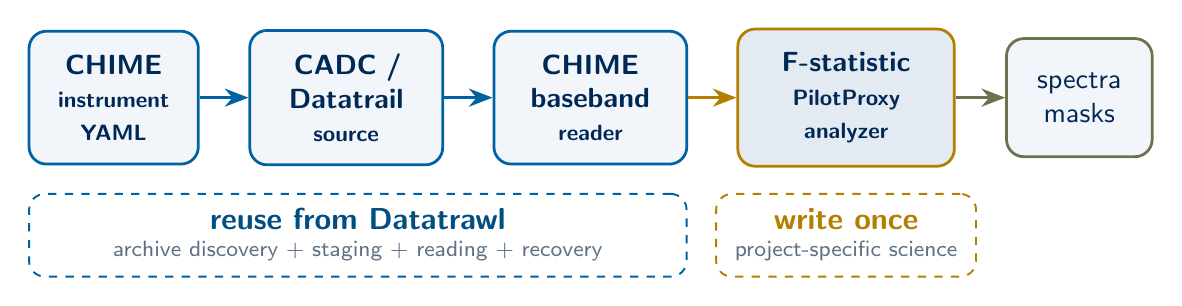
\begin{tikzpicture}[x=.92cm,y=.92cm]
    \node[card,minimum width=2.15cm,minimum height=1.5cm,text width=1.75cm,inner xsep=2mm] (inst) at (1.27,3.15)
      {\bfseries CHIME\\\fontsize{8.5}{10.5}\selectfont instrument YAML};
    \node[card,minimum width=2.45cm,minimum height=1.5cm,text width=2.05cm,inner xsep=2mm] (src) at (4.48,3.15)
      {\bfseries CADC / Datatrail\\\fontsize{8.5}{10.5}\selectfont source};
    \node[card,minimum width=2.45cm,minimum height=1.5cm,text width=2.05cm,inner xsep=2mm] (rdr) at (7.85,3.15)
      {\bfseries CHIME baseband\\\fontsize{8.5}{10.5}\selectfont reader};
    \node[cardamber,minimum width=2.75cm,minimum height=1.5cm,text width=2.35cm,inner xsep=2mm] (ana) at (11.38,3.15)
      {\bfseries F-statistic\\\fontsize{8.5}{10.5}\selectfont PilotProxy analyzer};
    \node[cardgreen,minimum width=1.75cm,minimum height=1.5cm,text width=1.45cm,inner xsep=2mm] (prod) at (14.6,3.15)
      {spectra\\masks};
    \draw[flow] (inst)--(src);
    \draw[flow] (src)--(rdr);
    \draw[flowamber] (rdr)--(ana);
    \draw[flowgreen] (ana)--(prod);

    \node[groupcyan,minimum width=8.35cm,minimum height=1.05cm] at (4.64,1.25) {};
    \node[text=DTCyanText,font=\fontsize{11}{13}\selectfont\bfseries] at (4.64,1.47)
      {reuse from Datatrawl};
    \node[text=DTMuted,font=\fontsize{8}{9.5}\selectfont] at (4.64,1.04)
      {archive discovery + staging + reading + recovery};
    \node[groupamber,minimum width=3.3cm,minimum height=1.05cm] at (11.38,1.25) {};
    \node[text=DTAmber,font=\fontsize{11}{13}\selectfont\bfseries] at (11.38,1.47)
      {write once};
    \node[text=DTMuted,font=\fontsize{8}{9.5}\selectfont] at (11.38,1.04)
      {project-specific science};
  \end{tikzpicture}
  \takeaway{For CHIME-compatible baseband, the science project normally supplies only the analyzer.}
  \source{README extension example: F-statistic DTV detector over 23 nominal pilots in event and scheduled baseband scopes.}
  \note{
    This is the payoff for the motivating PilotProxy campaign. The CHIME
    instrument geometry, the CADC/Datatrail source, and the CHIME baseband reader
    already exist. PilotProxy supplies the F-statistic analyzer as a plugin in
    the project that owns the scientific method. The analyzer can plan the 23
    nominal pilot selections and emit one or more resumable products. Datatrawl
    handles archive discovery, file staging, scratch cleanup, and recovery. This
    keeps detector changes independent of archive mechanics, and improvements to
    the engine benefit every analyzer rather than being copied between projects.
  }
\end{frame}

\section{Your first run}

% 22
\begin{frame}{Everything before survey runs without credentials}
  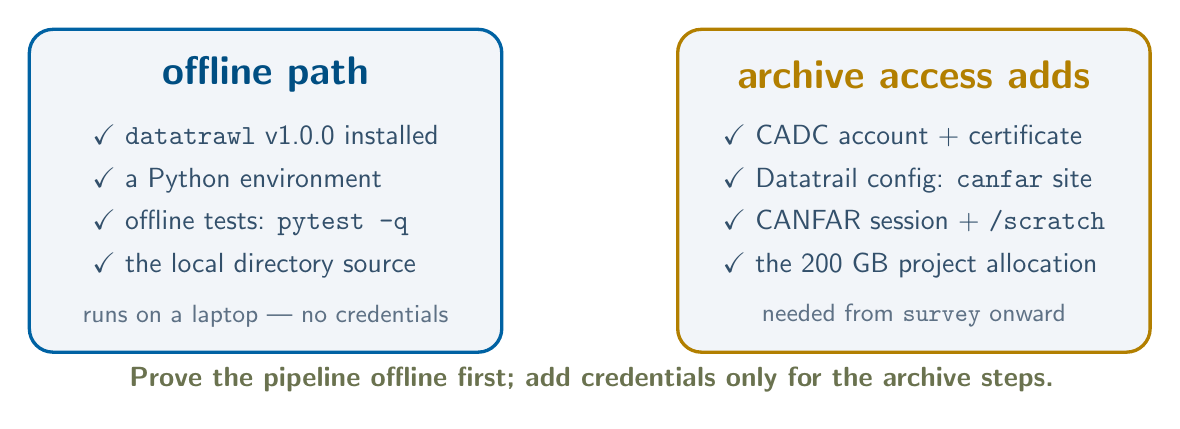
\begin{tikzpicture}[x=.92cm,y=.92cm]
    \node[panel,minimum width=6.0cm,minimum height=4.1cm] (offline) at (3.35,2.95) {};
    \node[panelhead] at (3.35,4.55) {offline path};
    \node[text=DTSoft,font=\fontsize{10.2}{12.5}\selectfont,align=left] at (3.35,2.8)
      {\checkmark\ \texttt{datatrawl} v1.0.0 installed\\[1mm]
       \checkmark\ a Python environment\\[1mm]
       \checkmark\ offline tests: \texttt{pytest -q}\\[1mm]
       \checkmark\ the local directory source};
    \node[text=DTMuted,font=\fontsize{9}{11}\selectfont] at (3.35,1.22)
      {runs on a laptop --- no credentials};

    \node[panelamber,minimum width=6.0cm,minimum height=4.1cm] (archivep) at (12.3,2.95) {};
    \node[panelhead,text=DTAmber] at (12.3,4.55) {archive access adds};
    \node[text=DTSoft,font=\fontsize{10.2}{12.5}\selectfont,align=left] at (12.3,2.8)
      {\checkmark\ CADC account + certificate\\[1mm]
       \checkmark\ Datatrail config: \texttt{canfar} site\\[1mm]
       \checkmark\ CANFAR session + \texttt{/scratch}\\[1mm]
       \checkmark\ the 200 GB project allocation};
    \node[text=DTMuted,font=\fontsize{9}{11}\selectfont] at (12.3,1.22)
      {needed from \texttt{survey} onward};

    \node[text=DTGreen,font=\fontsize{10}{12}\selectfont\bfseries] at (7.85,0.35)
      {Prove the pipeline offline first; add credentials only for the archive steps.};
  \end{tikzpicture}
  \takeaway{The offline path needs no credentials; add CADC and Datatrail access only when the tutorial reaches survey.}
  \source{Install and offline verification: repository README. Archive access: \texttt{cadc-get-cert}, \texttt{datatrail config init --site canfar}.}
  \note{
    Everything on the left runs on a laptop or in any CANFAR session with no
    credentials: install datatrawl from the repository README, run the offline
    test suite, and exercise the pipeline with the local directory source and
    synthetic data. The right column is needed only when we start touching the
    archive at the survey step: a CADC account with a valid certificate,
    Datatrail configured for the CANFAR site, and a session with scratch
    space. The full campaign additionally assumes our 200 GB project
    allocation. The next slide starts by proving the offline path.
  }
\end{frame}

% 23
\begin{frame}[fragile]{Start by proving the environment}
  \begin{tikzpicture}[x=.92cm,y=.92cm]
    \node[terminal,minimum width=8.3cm,minimum height=4.75cm,anchor=west] at (.35,2.75) {\begin{minipage}{7.65cm}
\begin{lstlisting}[style=dtterminal]
$ datatrawl --version
$ datatrawl list
$ datatrawl doctor
$ pytest -q

# Archive access only:
$ cadc-get-cert -u <user>
$ datatrail config init --site canfar
\end{lstlisting}
    \end{minipage}};

    \node[cardgreen,minimum width=4.9cm,minimum height=1.25cm] at (12.75,4.45)
      {\bfseries local pipeline verified};
    \node[card,minimum width=4.9cm,minimum height=1.25cm] at (12.75,2.75)
      {\bfseries plugins and\\combinations visible};
    \node[cardamber,minimum width=4.9cm,minimum height=1.25cm] at (12.75,1.05)
      {\bfseries archive credentials ready};
    \draw[flowgreen] (9.42,4.45)--(9.98,4.45);
    \draw[flow] (9.42,2.75)--(9.98,2.75);
    \draw[flowamber] (9.42,1.05)--(9.98,1.05);
  \end{tikzpicture}
  \takeaway{Separate an offline pipeline check from external archive readiness.}
  \source{Install and verification sequence: repository README. Offline tests and the local source require neither CADC credentials nor Datatrail configuration.}
  \note{
    The tutorial begins without touching the archive. Version confirms which
    release is installed. List shows the registered instruments, sources,
    readers, and analyzers, including external plugins. Doctor checks whether a
    requested combination is ready. The offline test suite exercises reader,
    analyzer, checkpoint, and resume paths with synthetic data. Only after this
    local path is proven do we add the CADC certificate and configure Datatrail
    for the CANFAR site. This separation makes failures diagnosable: a Python or
    plugin problem is not confused with a certificate, network, or archive
    problem.
  }
\end{frame}

% 24
\begin{frame}[fragile]{Survey and inspect before spending compute}
  \begin{tikzpicture}[x=.92cm,y=.92cm]
    \node[terminal,minimum width=9.0cm,minimum height=4.75cm,anchor=west] at (.25,2.65) {\begin{minipage}{8.35cm}
\begin{lstlisting}[style=dtterminal,basicstyle=\ttfamily\fontsize{9.6}{11.8}\selectfont\color{DTInk}]
$ datatrawl survey \
    --telescope chime \
    --source cadc-datatrail \
    --scope chime.event.baseband.raw \
    --freq-ids 844 --max-events 5 \
    --name chime-spectrum-844

$ datatrawl explore --name chime-spectrum-844
\end{lstlisting}
    \end{minipage}};

    \node[file,draw=DTGreen,minimum width=2.5cm,minimum height=1.55cm,
          font=\ttfamily\fontsize{8.2}{10}\selectfont] (inv) at (11.7,4.2)
      {inventory.jsonl};
    \node[file,draw=DTGreen,minimum width=2.5cm,minimum height=1.55cm,
          font=\ttfamily\fontsize{8.2}{10}\selectfont] (meta) at (11.7,1.8)
      {inventory.meta\\.json};
    \node[card,minimum width=2.1cm,minimum height=1.5cm,
          font=\fontsize{9.5}{12}\selectfont] (summary) at (14.45,3.0)
      {count\\volume\\date span};
    \draw[flowgreen] (10.03,3.6)--(inv.west);
    \draw[flowgreen] (10.03,2.2)--(meta.west);
    \draw[flow] (inv)--(summary);
    \draw[flow] (meta)--(summary);
  \end{tikzpicture}
  \takeaway{Build and inspect the work list before fetching the first bulk file.}
  \source{Current code resolves \texttt{--name} under \texttt{\$DATATRAWL\_INVENTORY\_ROOT} or \texttt{\string~/datatrawl-inventories/} by default;\\explicit \texttt{--out} still wins.}
  \note{
    This is the documented one-channel smoke survey. It selects the CHIME event
    baseband scope, frequency ID 844, and at most five not-yet-surveyed events.
    The name becomes the stable handle used by explore and scan. On current
    master, named inventories are written below DATATRAWL-INVENTORY-ROOT, or the
    datatrawl-inventories directory in the user's home by default, so the name
    resolves independently of the current working directory. Explore then prints
    the real unit count, volume, date span, and available frequency IDs. This
    survey is intentionally small; the full campaign would use the required
    scopes and selections without the smoke-test cap.
  }
\end{frame}

% 25
\begin{frame}[fragile]{Scan produces a resumable science product}
  \begin{tikzpicture}[x=.92cm,y=.92cm]
    \node[terminal,minimum width=8.2cm,minimum height=3.1cm,anchor=west] at (.25,3.65) {\begin{minipage}{7.55cm}
\begin{lstlisting}[style=dtterminal]
$ datatrawl scan \
    --name chime-spectrum-844 \
    --analyzer spectrum --select 844 \
    --max-frames-per-file 5
\end{lstlisting}
    \end{minipage}};
    \node[cardgreen,minimum width=5.6cm,minimum height=1.1cm] (npz) at (4.55,.95)
      {\texttt{results/chime/spectrum/844.npz}};
    \draw[flowgreen] (4.55,1.95)--(4.55,1.62);

    % Illustrative spectrum plot
    \draw[DTMuted,line width=.7pt] (10.1,1.15)--(10.1,4.95) (10.1,1.15)--(15.8,1.15);
    \node[text=DTMuted,font=\fontsize{8}{10}\selectfont,rotate=90] at (9.7,3.05) {power [relative]};
    \node[text=DTMuted,font=\fontsize{8}{10}\selectfont] at (12.95,.75) {sky frequency [MHz]};
    \draw[DTCyan,line width=1.0pt,smooth]
      plot coordinates {(10.1,1.65) (10.35,1.78) (10.6,1.55) (10.85,1.82)
      (11.1,1.62) (11.35,1.74) (11.6,1.57) (11.85,1.77) (12.1,1.65)
      (12.35,1.82) (12.6,1.72) (12.85,1.66) (13.05,1.75) (13.25,4.45)
      (13.42,1.88) (13.65,1.64) (13.9,1.76) (14.15,1.62) (14.4,1.84)
      (14.65,1.69) (14.9,1.78) (15.15,1.58) (15.45,1.73) (15.8,1.65)};
    \draw[DTAmber,line width=1.0pt,dashed] (13.25,1.15)--(13.25,4.7);
    \node[text=DTAmber,font=\fontsize{9}{11}\selectfont\bfseries,align=left,anchor=west]
      at (13.5,4.35) {candidate\\narrow feature};
    \node[text=DTMuted,font=\fontsize{8}{10}\selectfont] at (12.95,.25) {illustrative expected product};
  \end{tikzpicture}
  \takeaway{One command performs bounded staging, reading, analysis, cleanup, and checkpointing.}
  \source{README worked example. A feature near 470.309 MHz is an end-to-end path check, not a calibration or guaranteed detection.}
  \note{
    Scan reads the named inventory, infers its telescope, source, and reader, and
    runs the spectrum analyzer for frequency ID 844. The per-file frame cap makes
    this a fast end-to-end spot check even though each complete file is still
    fetched. The product is an NPZ under the analyzer's namespace, containing the
    accumulated PSD, count, frequency axes, provenance, and committed unit keys.
    If a retrievable selected event contains the DTV pilot, a narrow feature near
    470.309 megahertz is a useful path check. The plot here is illustrative, not
    measured data or an absolute calibration. A full uncapped product should use
    a fresh output; the analyzer rejects mixing capped and uncapped runs.
  }
\end{frame}

\section{Recovery}

% 26
\begin{frame}[fragile]{Recovery is intentionally boring: rerun the same command}
  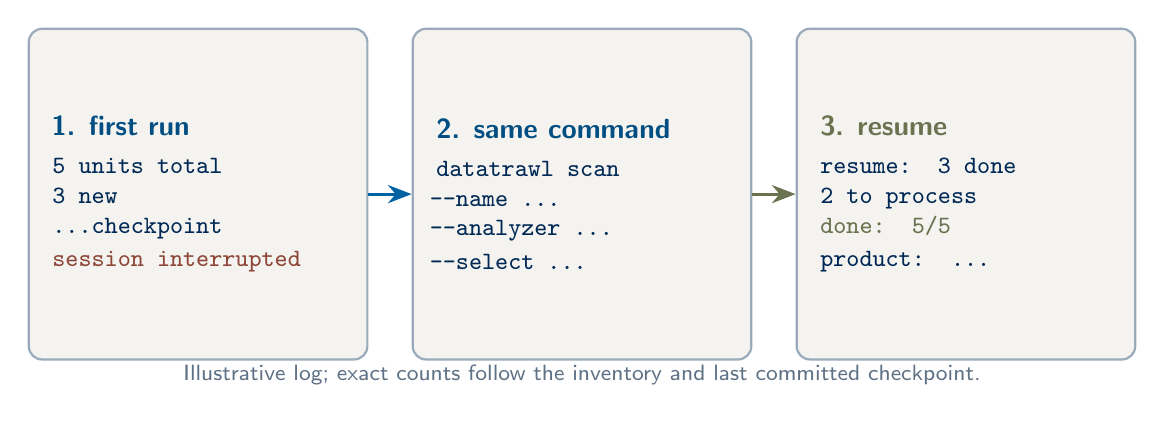
\begin{tikzpicture}[x=.92cm,y=.92cm]
    \node[terminal,minimum width=4.3cm,minimum height=4.2cm] (run1) at (2.5,2.65) {\begin{minipage}{3.7cm}
      {\color{DTCyanText}\bfseries 1. first run}\par\vspace{1mm}
      {\ttfamily\fontsize{8.6}{10.8}\selectfont
       5 units total\par
       3 new\par
       ...checkpoint\par
       \textcolor{DTRed}{session interrupted}}
    \end{minipage}};
    \node[terminal,minimum width=4.3cm,minimum height=4.2cm] (rerun) at (7.8,2.65) {\begin{minipage}{3.7cm}
      {\color{DTCyanText}\bfseries 2. same command}\par\vspace{1mm}
      {\ttfamily\fontsize{8.6}{10.8}\selectfont
       datatrawl scan\par
       --name ...\par
       --analyzer ...\par
       --select ...}
    \end{minipage}};
    \node[terminal,minimum width=4.3cm,minimum height=4.2cm] (resume) at (13.1,2.65) {\begin{minipage}{3.7cm}
      {\color{DTGreen}\bfseries 3. resume}\par\vspace{1mm}
      {\ttfamily\fontsize{8.6}{10.8}\selectfont
       resume: 3 done\par
       2 to process\par
       \textcolor{DTGreen}{done: 5/5}\par
       product: ...}
    \end{minipage}};
    \draw[flow] (run1)--(rerun);
    \draw[flowgreen] (rerun)--(resume);
    \node[sublabel] at (7.8,.15) {Illustrative log; exact counts follow the inventory and last committed checkpoint.};
  \end{tikzpicture}
  \takeaway{Normal recovery is the identical scan command; committed units are skipped and pending units are retried.}
  \source{README: ``To continue a run, repeat the same \texttt{scan} command with the same product-defining parameters.''}
  \note{
    The recovery procedure is intentionally simple. Run the same command with
    the same product-defining arguments. The analyzer loads the existing product,
    validates that the new run is compatible, and reports the committed unit
    keys. The engine excludes those keys from the to-do list. Fetch failures remain
    pending and are retried; quarantined keys remain excluded. For a controlled
    demonstration, use a fresh output and checkpoint every one or a few files,
    interrupt after a visible checkpoint, and repeat the command. Do not simulate
    recovery by changing the selection, frame cap, or scientific parameters.
  }
\end{frame}

% 27
\begin{frame}{The operator stops being the workflow engine}
  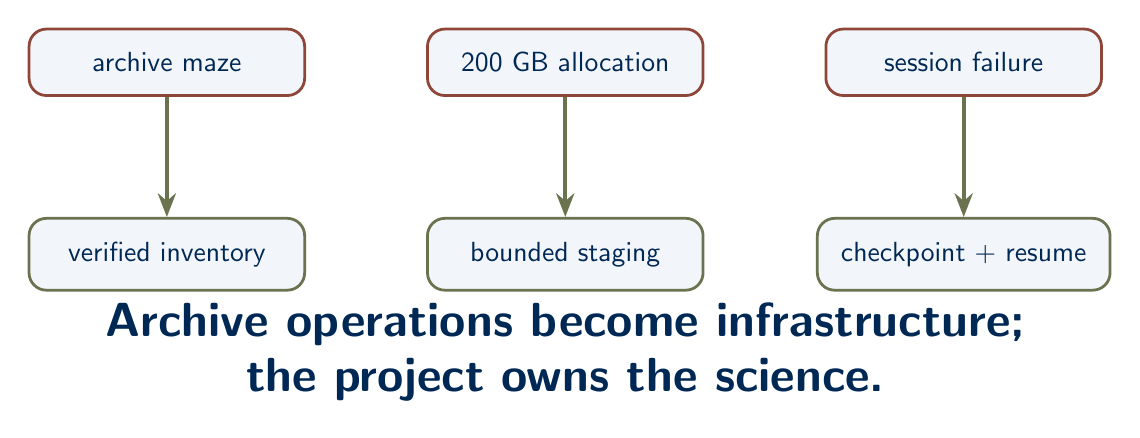
\begin{tikzpicture}[x=.92cm,y=.92cm]
    \node[cardred,minimum width=3.5cm] (maze) at (2.3,4.15) {archive maze};
    \node[cardred,minimum width=3.5cm] (quota) at (7.8,4.15) {200 GB allocation};
    \node[cardred,minimum width=3.5cm] (crash) at (13.3,4.15) {session failure};

    \node[cardgreen,minimum width=3.5cm] (inv) at (2.3,1.5) {verified inventory};
    \node[cardgreen,minimum width=3.5cm] (stage) at (7.8,1.5) {bounded staging};
    \node[cardgreen,minimum width=3.5cm] (resume) at (13.3,1.5) {checkpoint + resume};

    \draw[flowgreen,strong] (maze)--(inv);
    \draw[flowgreen,strong] (quota)--(stage);
    \draw[flowgreen,strong] (crash)--(resume);
    \node[text=DTInk,font=\fontsize{16}{20}\selectfont\bfseries,align=center]
      at (7.8,.15) {Archive operations become infrastructure;\\the project owns the science.};
  \end{tikzpicture}
  \takeaway{Datatrawl makes weeks-long archive processing bounded, auditable, and restartable.}
  \source{Datatrawl v1.0.0; tutorial grounded in \href{https://github.com/WVURAIL/datatrawl/tree/6d7a2391176b2828e6cee8fbffb5fee72311b6bf}{master @ 6d7a239}.}
  \note{
    We can now answer the three original motivations directly. The archive
    hierarchy becomes a verified, inspectable inventory. The 200-gigabyte
    allocation becomes an explicit maximum number of staged files. An unstable
    compute environment becomes a normal checkpoint-and-resume event rather than
    a reason to restart a weeks-long campaign. The result is not a larger science
    script. It is a boundary: archive operations become shared infrastructure,
    while PilotProxy or another project owns the scientific analyzer and its
    product. That is the reason Datatrawl is necessary and the standard workflow
    it establishes.
  }
\end{frame}

% 28
\begin{frame}{Rerun this tutorial, then bring your science}
  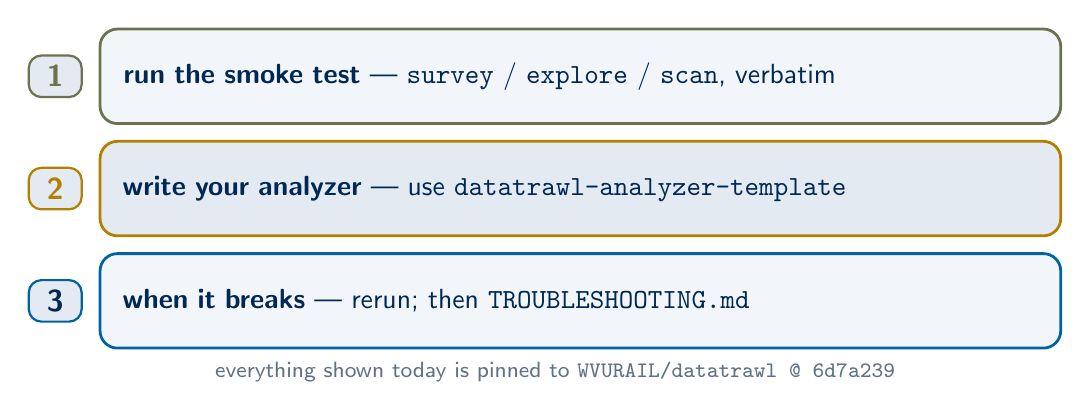
\begin{tikzpicture}[x=.92cm,y=.92cm]
    \node[chipgreen,font=\fontsize{11}{13}\selectfont\bfseries] at (1.15,4.4) {1};
    \node[cardgreen,anchor=west,align=left,text width=11.6cm,minimum height=1.2cm] at (1.75,4.4)
      {{\bfseries run the smoke test} --- \texttt{survey} / \texttt{explore} / \texttt{scan}, verbatim};
    \node[chipamber,font=\fontsize{11}{13}\selectfont\bfseries] at (1.15,2.85) {2};
    \node[cardamber,anchor=west,align=left,text width=11.6cm,minimum height=1.2cm] at (1.75,2.85)
      {{\bfseries write your analyzer} --- use \texttt{datatrawl-analyzer-template}};
    \node[chip,font=\fontsize{11}{13}\selectfont\bfseries] at (1.15,1.3) {3};
    \node[card,anchor=west,align=left,text width=11.6cm,minimum height=1.2cm] at (1.75,1.3)
      {{\bfseries when it breaks} --- rerun; then \texttt{TROUBLESHOOTING.md}};
    \node[sublabel] at (8.05,0.32)
      {everything shown today is pinned to \texttt{WVURAIL/datatrawl @ 6d7a239}};
  \end{tikzpicture}
  \takeaway{The smoke test is the on-ramp; a project plugs in as one analyzer; recovery stays the same command.}
  \source{Template: \href{https://github.com/WVURAIL/datatrawl-analyzer-template}{WVURAIL/datatrawl-analyzer-template}; contract: \href{https://github.com/WVURAIL/datatrawl/blob/6d7a239/docs/ADDING_AN_ANALYZER.md}{docs/ADDING\_AN\_ANALYZER.md}; \href{https://github.com/WVURAIL/datatrawl/blob/6d7a239/docs/TROUBLESHOOTING.md}{docs/TROUBLESHOOTING.md}.}
  \note{
    Three concrete next steps for the lab. First, rerun the tutorial yourself:
    the survey, explore, and scan commands shown today are copyable as-is, and
    the smoke caps keep a practice run cheap. Use your own inventory name so
    practice stays separate from campaign outputs. Second, when your project
    is ready, start from the analyzer template repository: use it as a
    GitHub template, rename the package, and replace the math. The entry
    point declared in its pyproject makes the analyzer first-class in list,
    doctor, and scan --- no extra flags --- and its offline test loop works
    before any archive access. The analyzer guide documents the contract;
    the supplied base class provides atomic saves and processed-key
    tracking, so most projects only write the science.
    Third, when something misbehaves, the first recovery tool is the one this
    tutorial ended with: rerun the same command with the same product-defining
    parameters; the troubleshooting guide covers certificates, sessions, and
    quarantine decisions. Bring questions to the group --- the deck and its
    backup slides are pinned to the exact commit, so references stay valid.
  }
\end{frame}

% =============================================================================
% Backup slides
\appendix

\begin{frame}{Backup: where durable state lives}
  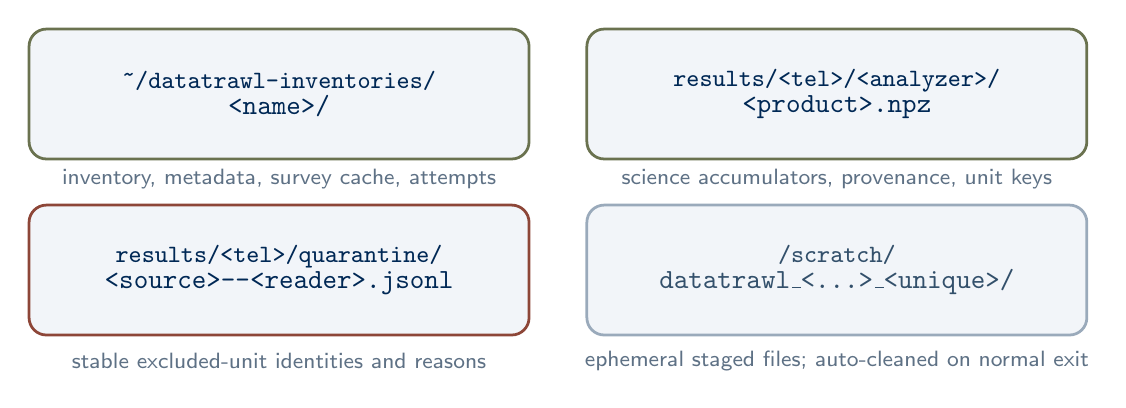
\begin{tikzpicture}[x=.92cm,y=.92cm]
    \node[cardgreen,minimum width=6.35cm,minimum height=1.65cm] at (4.05,4.15)
      {\fontsize{8.6}{10.5}\selectfont\texttt{\string~/datatrawl-inventories/}\\[-1mm]\texttt{<name>/}};
    \node[text=DTMuted,font=\fontsize{8.3}{10}\selectfont,align=center] at (4.05,2.98)
      {inventory, metadata, survey cache, attempts};

    \node[cardgreen,minimum width=6.35cm,minimum height=1.65cm] at (11.75,4.15)
      {\fontsize{8.6}{10.5}\selectfont\texttt{results/<tel>/<analyzer>/}\\[-1mm]\texttt{<product>.npz}};
    \node[text=DTMuted,font=\fontsize{8.3}{10}\selectfont,align=center] at (11.75,2.98)
      {science accumulators, provenance, unit keys};

    \node[cardred,minimum width=6.35cm,minimum height=1.65cm] at (4.05,1.72)
      {\fontsize{8.6}{10.5}\selectfont\texttt{results/<tel>/quarantine/}\\[-1mm]\texttt{<source>--<reader>.jsonl}};
    \node[text=DTMuted,font=\fontsize{8.3}{10}\selectfont,align=center] at (4.05,.47)
      {stable excluded-unit identities and reasons};

    \node[cardmuted,minimum width=6.35cm,minimum height=1.65cm] at (11.75,1.72)
      {\fontsize{8.6}{10.5}\selectfont\texttt{/scratch/}\\[-1mm]\texttt{datatrawl\_<...>\_<unique>/}};
    \node[text=DTMuted,font=\fontsize{8.3}{10}\selectfont,align=center] at (11.75,.47)
      {ephemeral staged files; auto-cleaned on normal exit};
  \end{tikzpicture}
  \takeaway{Inventories, products, and ledgers survive; the staging directory is disposable.}
  \note{
    Current master makes named inventories independent of the working directory.
    DATATRAWL-INVENTORY-ROOT can override the default under the user's home.
    Products remain under the current run root unless an explicit output path is
    provided. The quarantine ledger is scoped to the telescope plus source and
    reader. A unique scratch directory is created beneath DATATRAWL-TMPDIR, a
    writable scratch mount, or the operating-system temporary directory. Normal
    exit removes it. A hard kill can leave staged files behind; after confirming
    that no scan is using the directory, it can be removed.
  }
\end{frame}

\begin{frame}{Backup: explicit non-goals}
  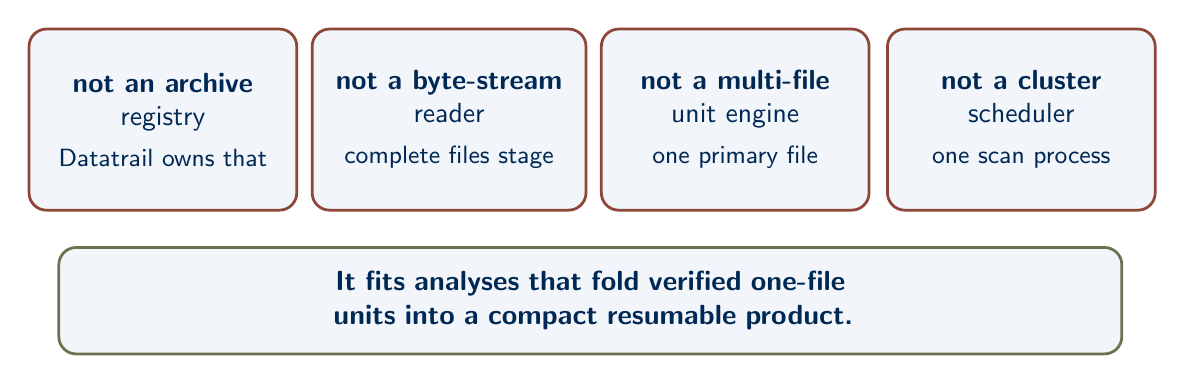
\begin{tikzpicture}[x=.92cm,y=.92cm]
    \node[cardred,minimum width=3.4cm,minimum height=2.3cm] at (2.2,3.35)
      {\bfseries not an archive\\registry\\[1mm]\fontsize{9}{11}\selectfont Datatrail owns that};
    \node[cardred,minimum width=3.4cm,minimum height=2.3cm] at (6.15,3.35)
      {\bfseries not a byte-stream\\reader\\[1mm]\fontsize{9}{11}\selectfont complete files stage};
    \node[cardred,minimum width=3.4cm,minimum height=2.3cm] at (10.1,3.35)
      {\bfseries not a multi-file\\unit engine\\[1mm]\fontsize{9}{11}\selectfont one primary file};
    \node[cardred,minimum width=3.4cm,minimum height=2.3cm] at (14.05,3.35)
      {\bfseries not a cluster\\scheduler\\[1mm]\fontsize{9}{11}\selectfont one scan process};

    \node[cardgreen,minimum width=13.5cm,minimum height=1.25cm,text width=12.5cm,
          font=\fontsize{10.3}{12.5}\selectfont] at (8.1,.85)
      {\bfseries It fits analyses that fold verified one-file units into a compact resumable product.};
  \end{tikzpicture}
  \takeaway{The explicit boundary is what makes the guarantees understandable.}
  \note{
    Datatrawl is intentionally narrow. It does not duplicate Datatrail's archive
    registration and storage policy. It does not consume archive objects as live
    byte streams; a complete file is staged. It does not present several primary
    files as one unit, although an analyzer can side-load a small companion using
    unit metadata. And it is not a distributed batch scheduler. These
    limitations are intentional. They define the model in which bounded
    staging, stable unit identity, and conservative resume behavior can be
    guaranteed.
  }
\end{frame}

\begin{frame}{Backup: recovery semantics}
  \begin{center}
  \fontsize{8.4}{10.2}\selectfont
  \setlength{\tabcolsep}{3.5pt}
  \renewcommand{\arraystretch}{1.24}
  \begin{tabular}{>{\RaggedRight\arraybackslash}p{2.15cm}>{\RaggedRight\arraybackslash}p{2.55cm}>{\RaggedRight\arraybackslash}p{2.9cm}>{\RaggedRight\arraybackslash}p{4.25cm}}
    \toprule
    \textcolor{DTCyanText}{\bfseries Failure} &
    \textcolor{DTCyanText}{\bfseries Run action} &
    \textcolor{DTCyanText}{\bfseries Unit on rerun} &
    \textcolor{DTCyanText}{\bfseries Why} \\
    \midrule
    Fetch fails & continue; count & pending; retry & transient faults may heal \\
    Probe fails & quarantine; continue & excluded by stable key & bytes arrived but are unreadable \\
    Reader fails mid-stream & quarantine; abort & excluded after restart & avoid ambiguous partial save \\
    Analyzer raises & abort; no quarantine & retry after analyzer fix & science error is not a bad-file verdict \\
    Survey service outage & preserve state; back off & resume same event & outage is not an empty dataset \\
    \bottomrule
  \end{tabular}\par
  \vspace{1mm}
  {\color{DTMuted}\fontsize{7.8}{9.5}\selectfont
    A custom analyzer is responsible for making its save/resume behavior equivalent to the supplied atomic base class.}
  \end{center}
  \source{\texttt{pipeline.py}, \texttt{analyzer\_base.py}, \texttt{cadc\_datatrail.py}.}
  \note{
    This table is the implementation-level reference for recovery semantics.
    The most important rule is that a completed unit is whatever the durable
    product says is completed. A log line, a successful download, or a partial
    accumulator update is not a commit. Survey applies the same conservative
    principle: a service it cannot reach is not interpreted as an empty scope or
    a file-free event. Partial survey state is preserved, and the same survey can
    continue after the service or credential recovers.
  }
\end{frame}

\begin{frame}{Backup: evidence base}
  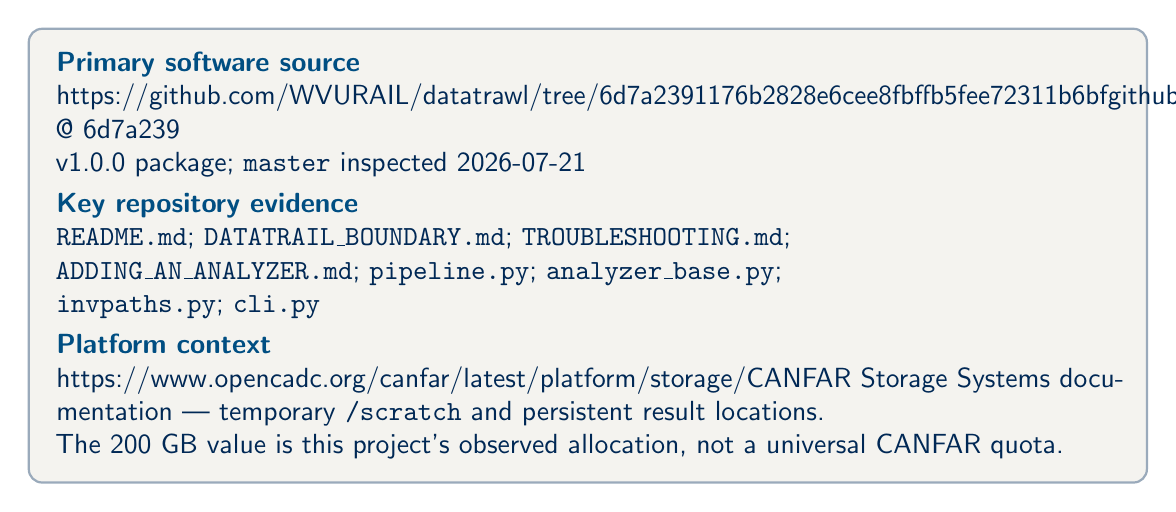
\begin{tikzpicture}[x=.92cm,y=.92cm]
    \node[terminal,minimum width=14.2cm,minimum height=4.2cm] at (7.83,2.65) {\begin{minipage}{13.5cm}
      {\color{DTCyanText}\bfseries Primary software source}\par
      \href{https://github.com/WVURAIL/datatrawl/tree/6d7a2391176b2828e6cee8fbffb5fee72311b6bf}{github.com/WVURAIL/datatrawl @ 6d7a239}\par
      v1.0.0 package; \texttt{master} inspected 2026-07-21\par\smallskip
      {\color{DTCyanText}\bfseries Key repository evidence}\par
      \texttt{README.md}; \texttt{DATATRAIL\_BOUNDARY.md}; \texttt{TROUBLESHOOTING.md};\\
      \texttt{ADDING\_AN\_ANALYZER.md}; \texttt{pipeline.py}; \texttt{analyzer\_base.py};\\
      \texttt{invpaths.py}; \texttt{cli.py}\par\smallskip
      {\color{DTCyanText}\bfseries Platform context}\par
      \href{https://www.opencadc.org/canfar/latest/platform/storage/}{CANFAR Storage Systems documentation} --- temporary \texttt{/scratch} and persistent result locations.\par
      The 200 GB value is this project's observed allocation, not a universal CANFAR quota.
    \end{minipage}};
  \end{tikzpicture}
  \takeaway{Every operational claim in the tutorial is tied to current code or current platform documentation.}
  \note{
    The deck is grounded in the live repository at the commit shown here, which
    was the tip of master when the presentation was created. The implementation
    files are the authority for the staging bound, checkpoint interval, failure
    classification, and inventory location. The official CANFAR documentation
    supports the distinction between temporary scratch and persistent storage.
    The 200-gigabyte number is deliberately labeled as our project's allocation,
    because quotas are account and allocation specific.
  }
\end{frame}

\end{document}
